%\documentclass[12pt]{article}
\documentclass[BCOR=12mm,DIV11,titlepage,a4paper,oneside]{scrbook}
\usepackage{scrhack}
\usepackage[ngerman]{babel}
\usepackage[utf8x]{inputenc}
\usepackage{amsmath}
\usepackage{graphicx}
\usepackage{caption}
\usepackage[colorinlistoftodos]{todonotes}
\usepackage{subcaption}

%fancyheadings funktioniert nicht mehr mit der KOMA Script Klasse scrbook

\usepackage{wrapfig}

\usepackage[authoryear,round]{natbib}

% Mittels [H] können Bilder genau an einer Stelle positioniert werden
\usepackage{float}

\usepackage[breaklinks]{hyperref}

% bewirkt das HyperLinks in der PDF nicht umrandet oder farbig sind
\hypersetup{colorlinks=false}

% package for colored text
% black,white,green,red,blue,yellow,cyan,magenta
\usepackage{color}
 
% package for colored tables
\usepackage{colortbl}

%Paket zur Erzeugung von Anführungszeichen durch \enquote{Text}
\usepackage[ngerman]{babel}
\usepackage[babel, german=quotes]{csquotes}

%Verhindern, dass eine neue Seite für ein einzelnes Wort/Zeile verwendet wird
\clubpenalty = 10000 % schliesst Schusterjungen aus 
\widowpenalty = 10000 % schliesst Hurenkinder aus (keine Beleidigung, sondern wirklich ein Fachbegriff)

\usepackage{lipsum}

\begin{document}

%!TEX root = ../main.tex
\begin{titlepage}

\begin{center}

% Logo der Technische Hochschule Köln
% Kann auch in dieser Form in Schwarz/Weiß ausgedruckt werden; Graustufen sollten der .tif Version entsprechen
\begin{figure}[!ht]
%	\centering
		
\includegraphics[width=0.26\textwidth]{images/THlogoheader.pdf}
\end{figure}

\vspace{0.4cm}

%Deutscher Titel
\begin{rmfamily}
\begin{huge}
\textbf{Wie zufriedenstellend ist ein System\\ für den Austausch von traditionellen und kulturellen Rezepten, \\wenn es nach der DIN-EN-ISO 9421-210,\\ für den Prozess zur Gestaltung gebrauchstauglicher interaktiver Systeme, konzipiert wird?}\\	
\end{huge}
\end{rmfamily}

\vspace{0.8cm}

%Englischer Titel
% \begin{rmfamily}
% \textbf{\LARGE Title in English}\\
% \large with a very\\long subtitle\\
% \normalsize
% \end{rmfamily}

% \vspace{1.2cm}

%Bachelorarbeit 
\begin{LARGE}
\begin{scshape}
Praxisprojekt\\[0.8em]
\end{scshape}
\end{LARGE}

%ausgearbeitet von...
\begin{large}
ausgearbeitet von\\ 
\vspace{0.3cm}
\begin{LARGE}
Joël Maximilian Mai\\
\end{LARGE}
\end{large}

\vspace{0.6cm}

%vorgelegt an der...
\begin{large}
vorgelegt an der\\ 
\vspace{0.2cm}
\begin{scshape}
Technischen Hochschule Köln\\
Campus Gummersbach\\
Fakultät für Informatik und\\
Ingenieurwissenschaften\\
\end{scshape}
\end{large}

\vspace{0.6cm}

%im Studiengang...
\begin{large}
im Studiengang\\ 
\vspace{0.1cm}
\textsc{Medieninformatik}
\end{large}


\vspace{1.2cm}

%Autor der Bachelorarbeit und die Prüfer
\begin{tabular}{rl}
        Prüfer:  &  Prof. Dr. Gerhard Hartmann\\
       					&  \small Technische Hochschule Köln \\[1.0em]
\end{tabular}

\vspace{1.2cm}

%Ort, Monat der Abgabe
\begin{large}
Gummersbach, im \Monat \the\year
\end{large}

\end{center}

\newpage
\thispagestyle{empty}

%Kontaktmöglichkeiten des Autors und der Prüfer
\begin{center}
\begin{tabular}{rl}
							&  \\[26.0em]
							
\large \textbf{Adressen:}	&  	\quad Joël Maximilian Mai\\
							&  	\quad Graf-Berghe-von-Trips-Ring 112\\
							&	\quad 50169 Kerpen\\
							&  	\quad joel\_maximilian.mai@smail.th-koeln.de\\[2.0em]
							
							&  	\quad Prof. Dr. Gerhard Hartmann\\
							&  	\quad Technische Hochschule Köln\\
							&  	\quad Institut für Informatik\\
							&	\quad Steinmüllerallee 1\\
							&	\quad 51643 Gummersbach\\
							&  	\quad gerhard.hartmann@th-koeln.de\\[2.0em]
\end{tabular}
\end{center}

\end{titlepage}

\pagenumbering{Roman}
\tableofcontents
\addcontentsline{toc}{chapter}{Inhaltsverzeichnis}
\setcounter{page}{1}
\newpage

\chapter*{Kurzfassung}
\addcontentsline{toc}{chapter}{Kurzfassung}
% Basic introduction to the field - verständlich für jeden Wissenschaftler jedes Feldes

% 2-3 Sätze zu mehr detailierten Hintergrund - verständlich für MCIler

% 1 Satz das Problem addressieren

% 1 Satz das Ziel zusammenfassen

% 2-3 Sätze wie das Endergebnis im Vergleich zu bisherigen Wissenstand zu diesem beiträgt/erweitert

% 1-2 Sätze wie die Ergebnisse in einen gernerellen Kontext passt

% 2-3 Sätze für eine Breitere Perspektive 

\newpage
\chapter*{Abstract}
\addcontentsline{toc}{chapter}{Abstract}
Hier folgt die Kurzfassung auf Englisch. Wenn Sie diese Vorlage für Seminararbeiten, Projektdokumentation o.ä. verwenden ist eine englische Kurzfassung ggf. nicht nötig.

\newpage
\pagenumbering{arabic}
\chapter{Einleitung}
\label{cha:Einleitung}

\section{Herausforderung und Motivation}
\subsection{Wirtschaftliche Relevanz}
% die Anpassung einer Gestaltung an die Erfordernisse und Fähigkeiten der Benutzer verbessert deren Nutzung, Qualität und Effizienz, wodurch preisgünstige Gestaltungslösungen zur Verfügung gestellt werden und die Wahrscheinlichkeit reduziert wird, dass Systeme, Produkte und Dienstleistungen unwirtschaftlich sind oder von ihren Benutzern abgelehnt werden; 
Bestehende Implementierungen eines Systems, das die beschriebenen Use Cases abdecken soll, mangelt es an Qualität der Benutzbarkeit und erfüllen nicht die erhobenen Anforderungen der Stakeholder. So sind zum Beispiel 52\% der Nutzer sehr unzufrieden mit der größten Rezepteplattform Chefkoch \citep{trustpilot:online}. Software Dienstleistungen werden durch Werbung finanziert \citep[vgl. Punkt 1]{HowDoFre38:online}. Diese Werbung wirkt auf den Nutzer tendenziell ablenkend und wird als störend während des Kochens oder Stöberns wahrgenommen \citep{Allesvol19:online}. Durch die Nutzung von Online Foren und großen internationalen Restaurantketten geraten die lokalen Rezepte der Familie in den Hintergrund \citep{bpb2021fastfood, bpb2021fastfoodtopic, HowHasGl49:online}. Die Implementierung der Rechtefreigaben für eigene Rezepte ist mangelhaft. Es muss gegeben sein, dass Nutzer entscheiden können welche Rezepte öffentlich, mit der Familie geteilt oder privat sind.\\
Hier bedarf es eines Systems, welches die oben gelisteten Punkte adressiert. 

\subsection{Wissenschaftliche Relevanz}
Zur Zeit der Ausarbeitung ist die Etablierung von Progressiven Web Applikationen (kurz PWA) stagniert \citep{Magomadov_2020}. Im Gegensatz zu nativen Applikationen bieten PWAs den Vorteil, dass sie auf jedem Endgerät mit einem Browser installiert werden können, je nach Endgerät und genutztem Browser mit Einschränkungen in den Funktionalitäten \citep{MScthesi20:online, Progress77:online}. \\
Jedoch bringt die Implementierung einer App, ob nativ oder als Web App, für verschiedene Betriebssysteme das Problem mit sich, sodass das User Interface nach den unterschiedlichen Design Guidelines zu gestalten ist \citep{Mitrovic2016ARO}. Hier bedarf es einer Lösung, die auf allen Betriebssystemen von allen Nutzern als ergonomisch bewertet wird. Dementsprechend müssen aktuelle Guidelines untersucht und eine Gestaltungslösung umgesetzt werden, welche die Vorgaben in einem eigenen Styleguide bündelt.\\
Ein System das von Nutzern befüllt und genutzt wird, bedarf besonderer Konzeption in Hinsicht auf Datenschutz und Barrierefreiheit \citep{Privacya9:online}. Im Rahmen der Gestaltung und Architektur soll hier ein Konzept entwickelt werden, welches die Bereiche zufriedenstellend abdeckt.

\subsection{Soziologische Relevanz}
% ein menschzentrierter Ansatz führt zu Systemen, Produkten und Dienstleistungen, die besser für die Gesundheit, das Wohlbefinden und das Engagement ihrer Benutzer sind, einschließlich der Benutzer mit Behinderungen.
Aufgrund der Globalisierung ist die Wahrung und Förderung von Kultur und Tradition eine wichtige Aufgabe \citep{BryanTurner_2016}. Erreicht wird dieses Ziel durch die vereinfachte Weitergabe von Wissen an kommende Generationen. Durch die Dokumentation von Familienrezepten wird aber auch die kritische Auseinandersetzung mit der eigenen Vergangenheit angeregt \citep{76f9434be2ae4e23b9f44d93097c915c}. Zusätzlich werden aus fachlichen Kochbüchern, angereichert durch persönliche Anekdoten, Werke von emotionalem Wert.

\section{Bezug zum Entwicklungsprojekt}
Es wurde bereits im Rahmen des Entwicklungsprojekts \citep{cobanmai2021} ein vertikaler Prototyp entwickelt, welcher die Umsetzbarkeit eines Systems auf Basis der Technologie PWA und Peer to Peer bewertet hat. Die Artefakte dieses Projekts wurden teilweise mit in die Konzeption dieses interaktiven Systems mit eingebracht. Das Einverständnis des Teammitgliedes des Entwicklungsprojekts für die Nutzung der Artefakte liegt vor.

\section{These}
Diese Arbeit setzt sich mit der Gestaltung interaktiver Systeme auseinander, die anhand der DIN-EN-ISO 9421-210 \citep{DINISO_2010} erarbeitet wurden. Es soll festgestellt werden, ob die Qualität der erarbeiteten Gestaltungslösung, für ein System das den Austausch von traditionellen und kulturellen Rezepten ermöglicht, den Nutzererwartungen und Ansprüchen an die Gebrauchstauglichkeit und Ergonomie entspricht.
Es soll festgestellt werden, ob es einen Zusammenhang zwischen der früh durchgeführten Evaluierung und Iteration der Gestaltungslösung und der Zufriedenheit der Nutzer auch im Bezug auf dieses System besteht.
Desweiteren soll festgestellt werden, welchen Einfluss die Auswahl der Nutzergruppe und die Integration dieser auf die Konzeption des Systems haben.

\newpage
\chapter{Hauptteil}
\label{cha:Hauptteil}
\section{Umsetzung}
\subsection{Verstehen und Festlegen des Nutzungskontexts}
Für die Roadmap der Anforderungsermittlung wurde das Vorgehen der DIN-EN-ISO 9241-210 gewählt. Für die Konzeption eines best möglichen Systems wurde hier von den bisherigen Erkenntnissen zurück getreten und lösungsneutral an das Domänenmodell herangegangen.
% Vollständig, Notwendig, Atomar, Verfolgbar, Technisch lösungsneutral, Realisierbar, Konsistent, Eindeutig, Prüfbar, Vollständig, Konsistent, Erschwinglich, Abgegrenzt, Schnittstellenanforderung

\subsubsection{Domänenmodell}
\begin{figure}[h] %!=overrides latex; h=here; t=top; b=bottom; p=special page for floating objects
    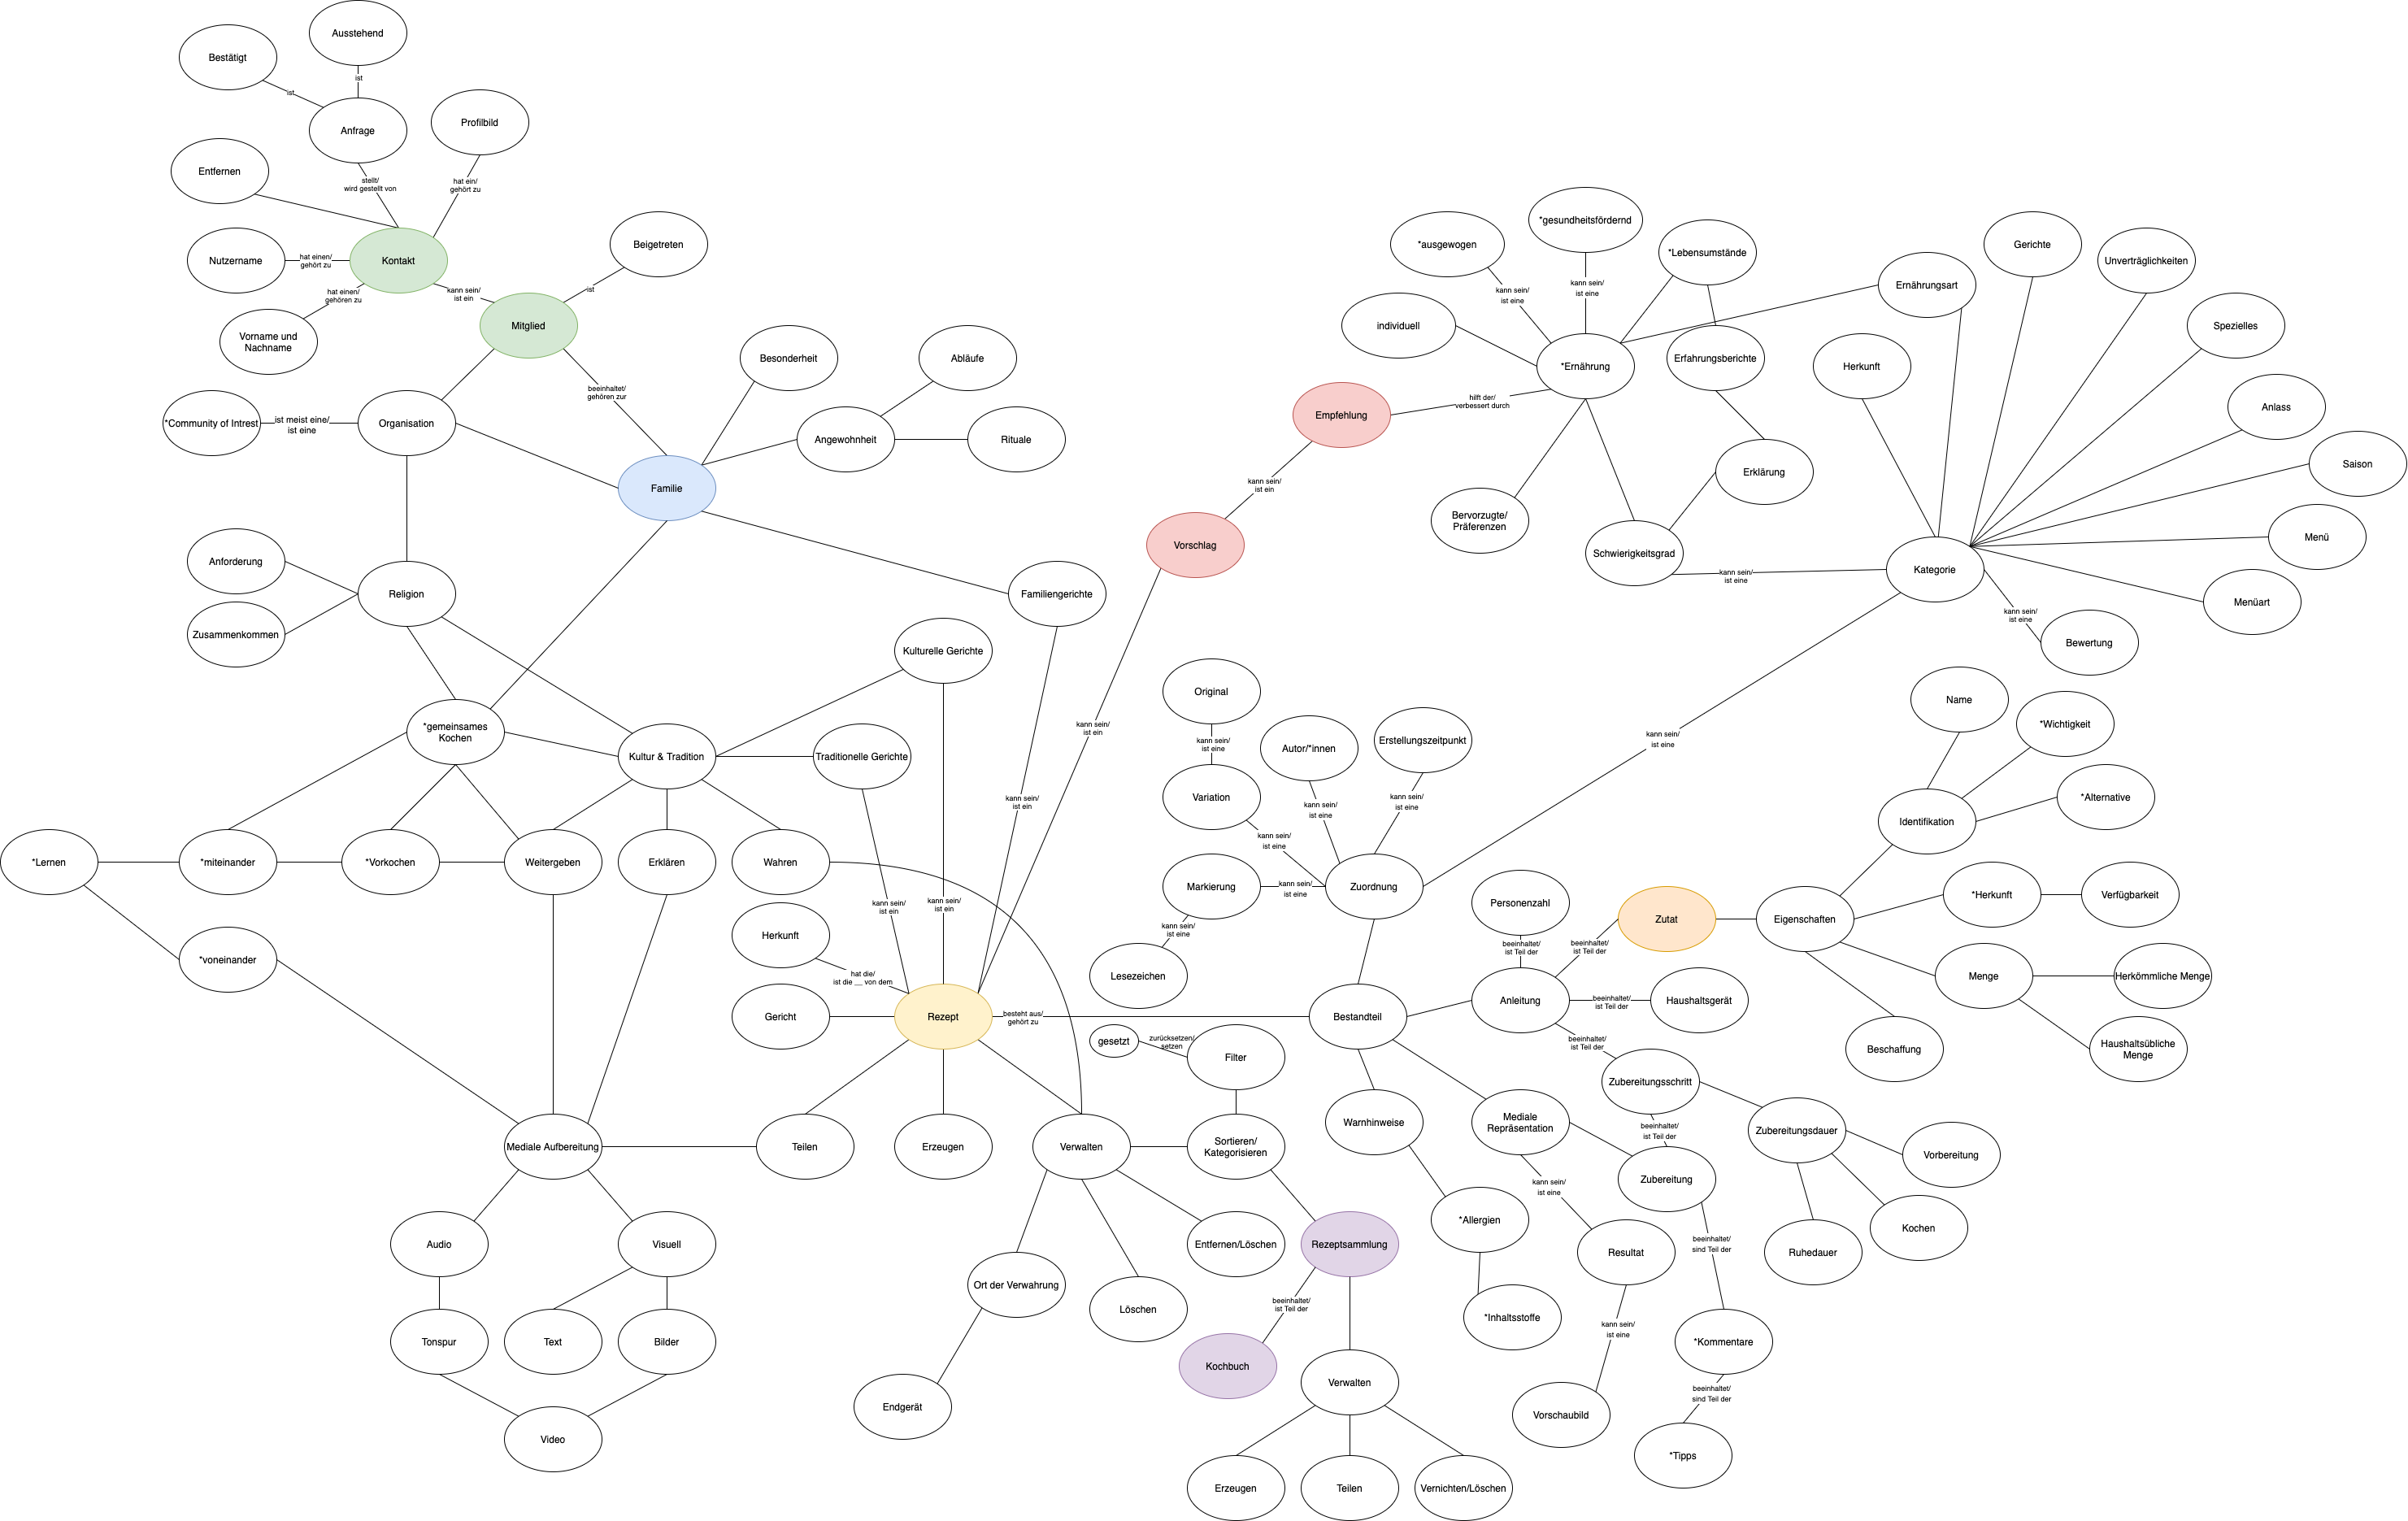
\includegraphics[width=1\textwidth]{images/domainmodel.png}
    \caption[Domänenmodell]{Domänenmodell}
    \label{fig:Domaenenmodell}
\end{figure}
Neben den offensichtlichen Domänenen wie Kochen, Rezepte, Tradition, Kultur und Familie ergeben sich hier auch die Erweiterung des Modells durch Religion und Zutateneigenschaften wie zum Beispiel die Verträglichkeit als auch Ernährung. Durch die Aufteilung verschiedener Domänen ergab sich auch die Aufteilung von Zubereitung in Zubereitungsschritt und die daraus sich zusammen addierbare Zubereitungsdauer. Haushaltsgeräte für jedes Rezept aufzulisten, ist ebenfalls eine Idee als Funktion die erst mit Hilfe der Erstellung eines Domänenmodells ermöglicht wurde. Auch die Unterscheidung von Vorschlag und Empfehlung ergab sich aus dem Modell.\\

\subsubsection{Festlegen der Nutzeranforderungen}
\label{sec:userstories}
\begin{figure}[h] %!=overrides latex; h=here; t=top; b=bottom; p=special page for floating objects
    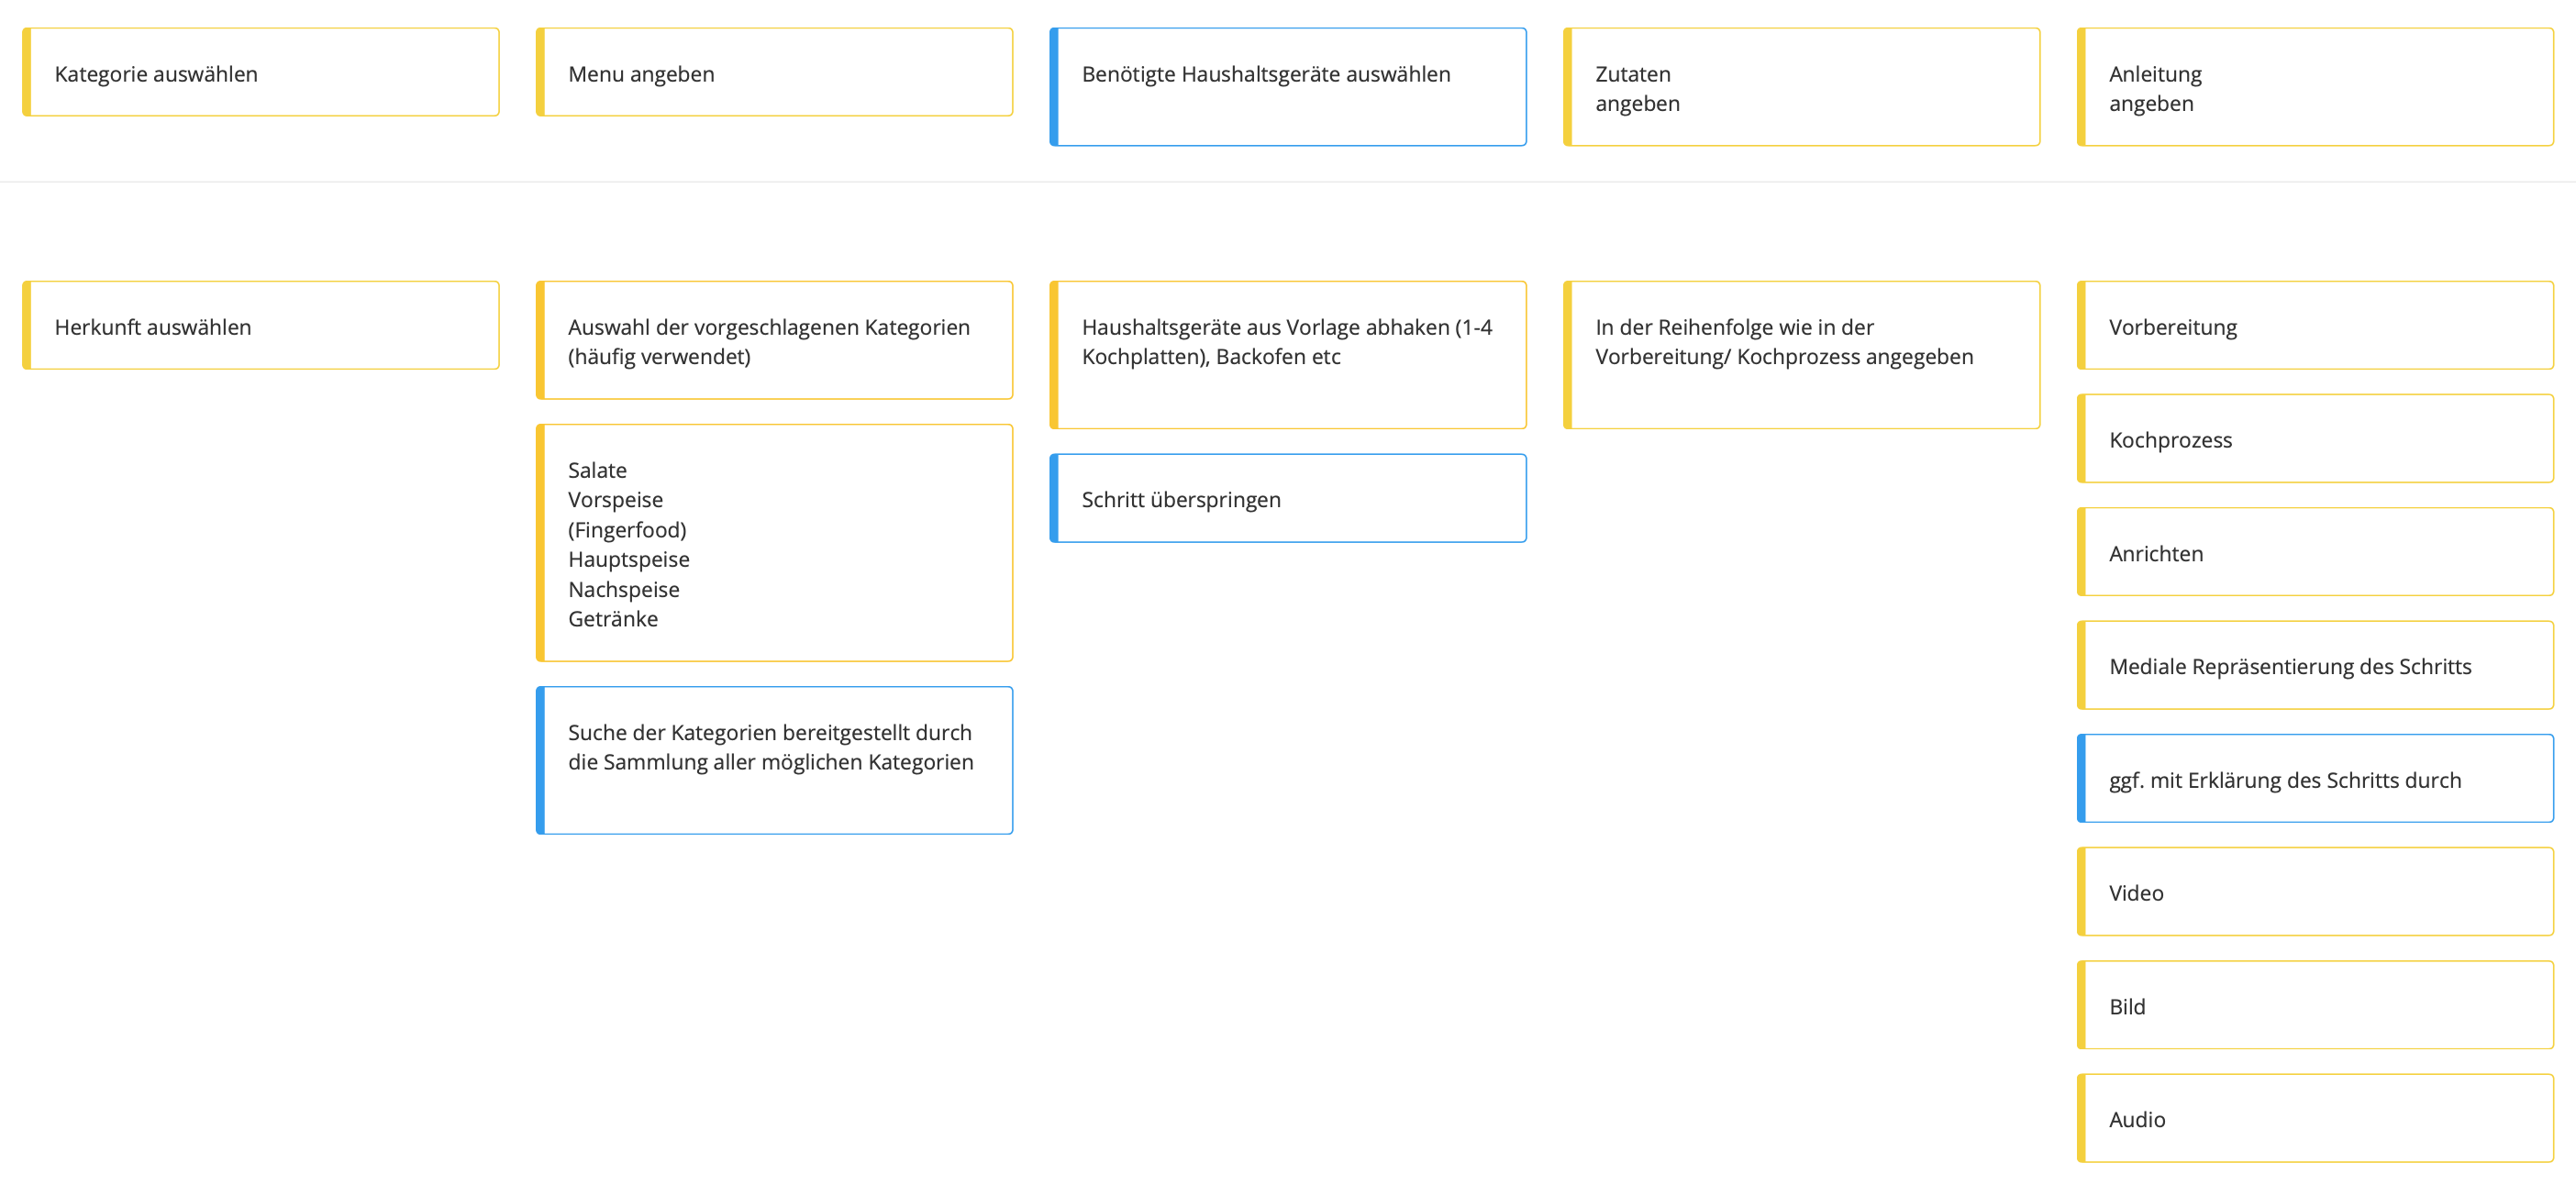
\includegraphics[width=1\textwidth]{images/userstories.png}
    \caption[User Stories (Ausschnitt)]{User Stories (Ausschnitt)}
    \label{fig:userstories}
\end{figure}
Um später bestimmen zu können ob die Anforderungen erfüllt worden sind, wurde mit den potentiellen Nutzern ein Workshop zur Erarbeitung der User Stories und die Priorisierung für den MVP abgehalten. Anhand der User Stories ergab sich zum einen die geringe Wichtigkeit und Bedeutung von Datenschutz im Sinne der Lokalisierung der Daten der jeweiligen Nutzern. Für sie war eine verschlüsselte Datenbank unabhängig von großen Konzernen wie Google und Amazon ausreichend. Des Weiteren wurden die Titel der einzelnen Schwierigkeitsgrade festgelegt (Einfach, Normal, Anspruchsvoll). Zusätzlich zu aufgeteilten Angabe der Zubereitungsdauer (Vorbereitung, Zubereitung, Anrichten), soll auch die Backzeit, Temperatur des Backofens als auch die Einstellung angegeben werden können. Durch vordefinierte Kategorien soll die Zuordnung und das Wiederfinden erleichtert werden. Haushaltsgeräte anzugeben soll übersprungen werden können. Die Angabe von Zutaten soll mit einem Hinweis erweitert werden, die Zutaten auch in der Reihenfolge anzugeben, wie sie auch in der Zubereitung verwendet werden. Rezepte sollen als Privat markiert werden können und dem entsprechend nicht von anderen eingesehen werden können. Weniger wichtige Punkte waren die automatische Generierung von Kalorien und Inhaltsstoffe der Zutaten. Besonders wichtig und von allen Teilnehmern gewünscht ist die Funktion, dass der Bildschirm sich während des Kochens nicht abschaltet, um die Lesbarkeit der Zubereitungsschritte zu gewährleisten. Im Nachgang an den Kochprozess oder bei dem Anlegen eines Rezepts können von Nutzern persönliche Anekdoten, Tipps und Tricks oder einfach Kommentare verfasst werden. Um die Veränderungen in Familienrezepten über mehrere Generation besser nachvollziehen zu können, werden sowohl das Originalrezept, als auch den Vorgänger des aktuell betrachteten Rezepts dem Nutzer präsentiert.
 % Zuweisen von Ressourcen, sowohl um frühzeitige Rückmeldungen zur Verbesserung des Produkts zu erhalten als auch, in einer späteren Phase, um zu bestimmen, ob die Anforderungen erfüllt wurden;
% --> Use–Case–Modellierung

\subsubsection{Content und Navigation Map}
\begin{figure}[h] %!=overrides latex; h=here; t=top; b=bottom; p=special page for floating objects
    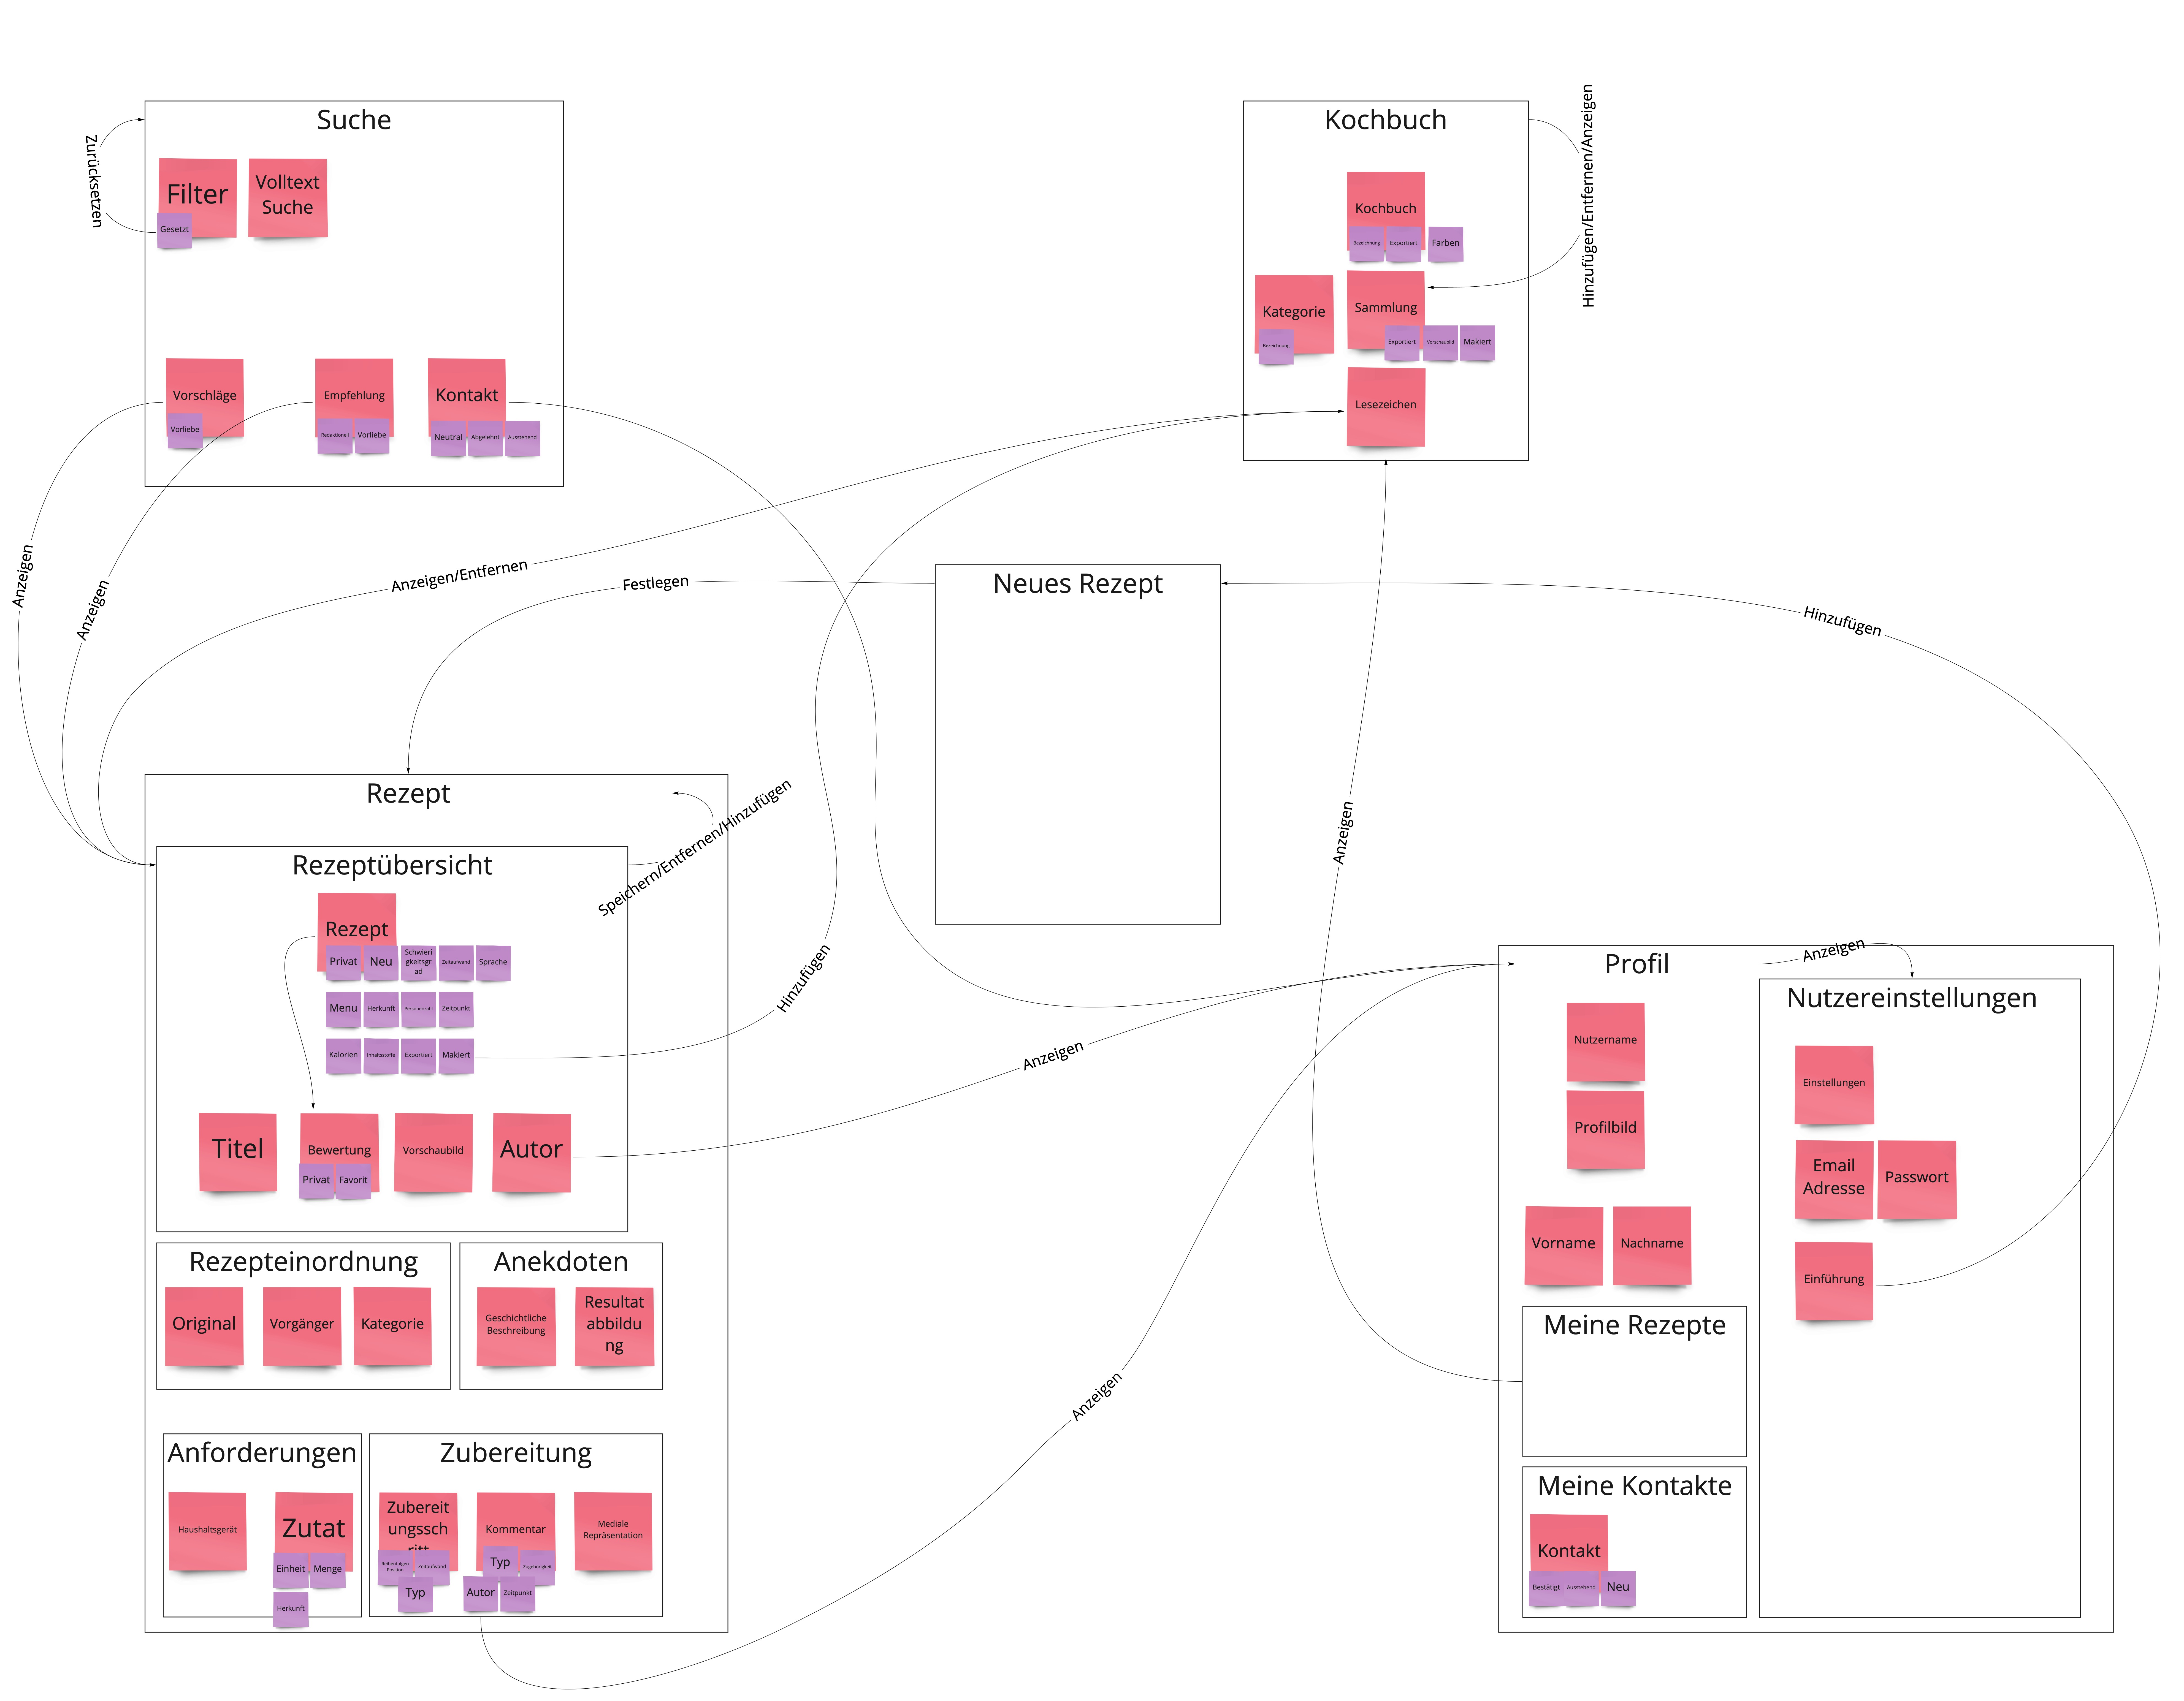
\includegraphics[width=1\textwidth]{images/navigationmap.jpg}
    \caption[Content Map erweitert zur Navigation Map]{Content Map erweitert zur Navigation Map}
    \label{fig:navigationmap}
\end{figure}
Um die Navigation des Systems so selbsterklärend wie möglich zu gestalten, wurden die User Stories nach Content Objekten gefiltert und diese um die Duplikate in den verschiedenen Clustern reduziert. 
% Hier ergänzen wie das Verfahren genannt wird und von wem es kam
Anschließend wurden zwischen den Objekten durch die erhaltenen Verben Verbindungen gezogen die später die Navigationswege darstellen sollen. Zusätzliche Objekte oder Zustände wurden in lila Karten dargestellt und zu den jeweiligen Objekten angeheftet. Neben klar geclusterten Gruppen wie Kochbuch, Suche und Neues Rezept stellte sich die Clusterung des Rezepts als Herausforderung hervor. Da hier die Einteilung in Untergruppen besonders schwierig war. Das Cluster Rezeptübersicht soll wesentliche Informationen eines Rezepts beeinhalten, jedoch nicht die einzelnenen Schritte eines Rezepts da diese die Übersicht überladen würden. Die Rezepteinordnung hat im wesentlichen nichts mit dem eigentlichen Rezept zu tun, daher wird auch sie getrennt von dem Rezept und in ein eigenes Cluster verschoben. Für die Anekdoten gilt selbiges. Die Anforderungen beeinhalten die Zutaten und Haushaltsgeräte und sind für die Zubereitung zwar wesentliche Bestandteile jedoch keine Zubereitungsschritte. Daraus ergibt sich das letzte Cluster Zubereitung. Hierzu gehört der Zubereitungsschritt, dessen Position in der Zubereitungsreihenfolge, der Zeitaufwand, und die Bezeichung/Typ des Schritts. Zu diesem Zeitpunkt war geplant das für jeden Schritt einzelne Mediale Repräsentationen hinzugefügt werden können aber auch das jeweils Kommentare und die dazu gehörigen Typen von Kommentaren zu jedem Schritt hinzugefügt werden könnnen. Dieser Gedanke wurde jedoch wieder verworfen, einerseits durch die Reduzierung der Funktionen des MVPs aber auch durch Evaluierung anhand der potentiellen Nutzergruppe. Das Profil ist in die Übersichtsobjekte eines Profils unterteilt und erweitert durch die eigenen Rezepte, die besonders hervorgehoben werden sollen oder als Empfehlung gekennzeichnet sind, und die Kontakte die dieses Profil hält. Aus der Recherche hat sich ergeben, dass die meisten sozialen Dienste die Einstellungen zu dem eigenen Konto oder der Applikation meistens auch in der Profilansicht anordnen. Daher ist es naheliegend um die Lernbarkeit des Systems zu gewährleisten auch hier die Einstellungen zum Profil anzuordnen. \\
% Erläutern, warum einzelne Empfehlungen nicht anwendbar sind;

\subsection{Erarbeitung von Gestaltungslösungen zur Erfüllung der Nutzungsanforderungen}
Anhand der Content Map und der dort erarbeiteten Cluster sollen nun im Zusammenspiel mit der Navigation Map Gestaltungslösungen erarbeitet werden die die Nutzeranforderung erfüllen. Dabei wurde in jedem Schritt eine Evaluierung durchgeführt und Alternative Lösungen präsentiert. Anhand der Auswahl der Nutzergruppen wurde somit die richtige Gestaltungslösung erarbeitet.
% Kurz die Roadmap erklären und das einbeziehen/den Einbezug der Nutzergruppe

\subsubsection{Wireframes}
\begin{wrapfigure}{r}{0.4\textwidth}
  \centering
    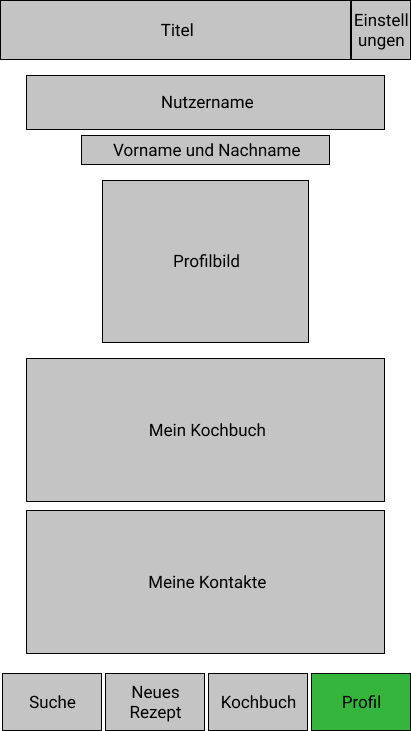
\includegraphics[width=0.28\textwidth]{images/wf-profil.jpg}
  \centering
\caption[Wireframe - Profil]{Wireframe - Profil}
\label{fig:wf-profil}
\end{wrapfigure}
Für die Gewährleistung der Konformität der Benutzererwartungen wurden die Cluster aus der Navigation Map möglichst nach Priorität für die Nutzer auf den verschiedenen Endgeräten angeordnet. Auf der Abbildung \ref{fig:wf-profil} erkennt man deutlich die Cluster aus der Abbildung \ref{fig:navigationmap} wieder. Im oberen Bereich, welcher auf den ersten Blick am besten gelesen werden kann, sind die Informationen die für das Cluster am wichtigsten waren, angeordnet. Die Navigation, welche die wahrscheinlich häufigste Interaktion zu erwarten hat befindet sich für den Nutzer am leichtesten erreichbar an dem unteren Bildschirmrand. Ganz oben am Bildschirmrand, mit der wahrscheinlich wenigsten Interaktion im Alltagsgebrauch befindet sich die Titelleiste ergänzt um die Einstellungen. \\ Das selbe Verfahren wurde für die übrigen Wireframes verwendet und von den Nutzern als zufriedenstellend bewertet. \\
% Konformität mit Benutzererwartungen

\subsubsection{Styleguide}
Um an die Gestaltung traditioneller Kochbücher anzulehnen wurde noch vor der Gestaltung einzelner Screens, die Farbpalette und Schriftarten gewählt. Für die Farbpalette wurden verschiedene Fotografien von Gerichten auf ihre Farben analysiert und auf typische Farbpaletten aus der Webseitengestaltung wie zum Beispiel Bootstrap abgebildet. Das ergibt die primären Farben des Systems.  \\
\begin{figure}[h] %!=overrides latex; h=here; t=top; b=bottom; p=special page for floating objects
    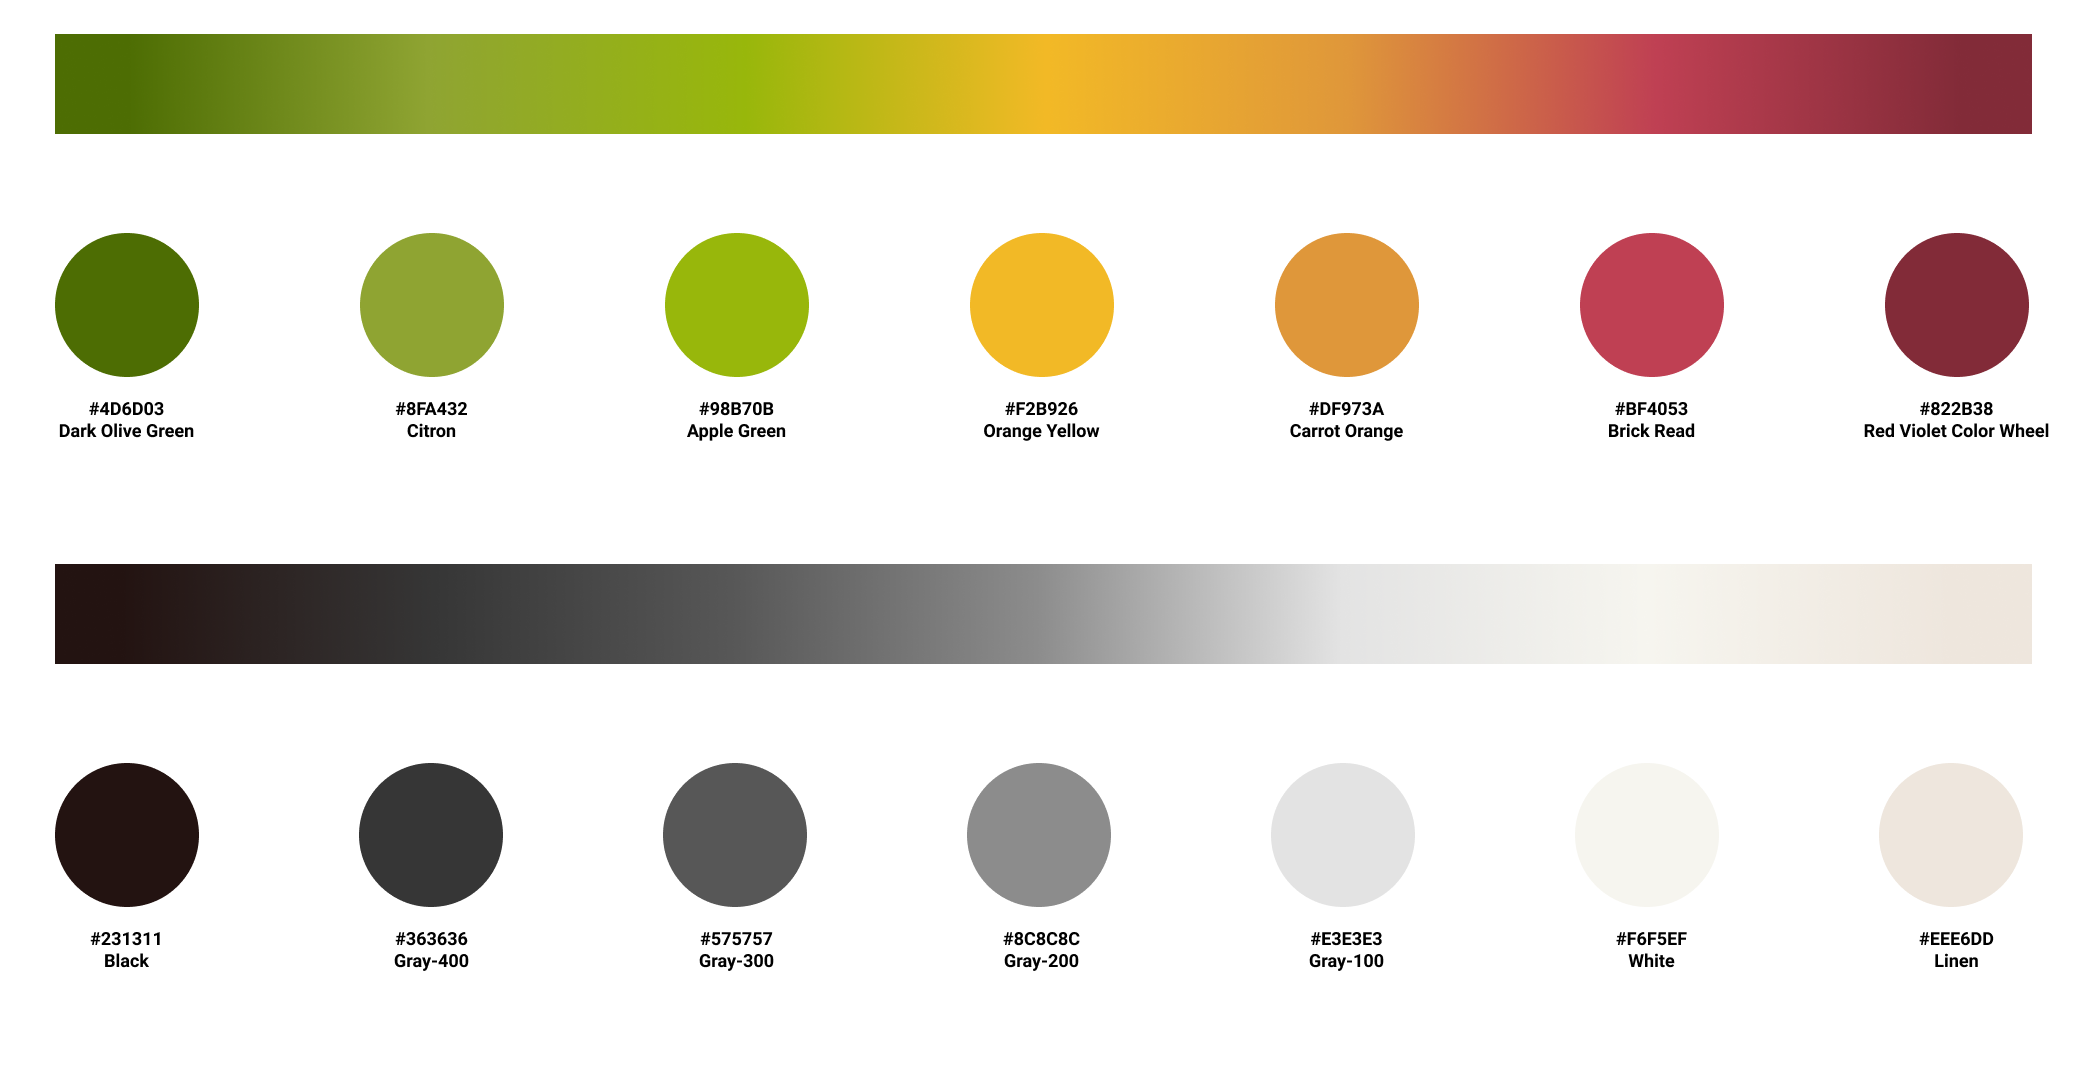
\includegraphics[width=1\textwidth]{images/colorscheme.png}
    \caption[Farbschema für den Styleguide]{Farbschema für den Styleguide}
    \label{fig:styleguide-colorscheme}
\end{figure}
\\
\begin{wrapfigure}{r}{0.4\textwidth}
  \centering
    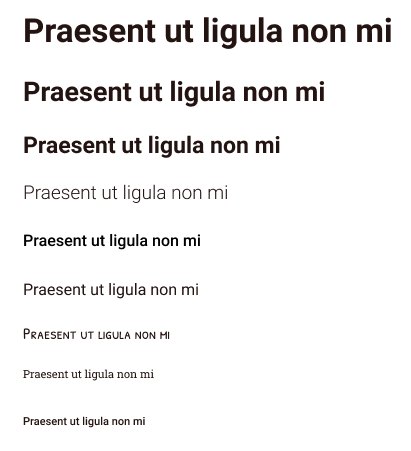
\includegraphics[width=0.4\textwidth]{images/typographie.png}
  \centering
\caption[Typographie]{Typographie}
\label{fig:styleguide-typographie}
\end{wrapfigure}
Für die Schriftarten wurden freie Schriftarten auf ihre charakteristischen Eigenschaften analysiert und anhand eines Rezeptes getestet um für verschiedene Aufgaben auch die korrekte Schriftart zu wählen. Nutzern wurde diese verschiedenen Lösungen präsentiert und dann evaluiert. Ein wichtiger Einwand ist hier die Verfügbarkeit dieser Schriften, da sie mit jeder Nutzung auch heruntergeladen werden müssen. Letztendlich wurden verschiedene Schriftfamilien für das System ausgewählt. \\
Um die Erstellung der Gestaltungslösungen zu erleichtern wurde nach dem Atomic Design eine Styleguide erarbeitet der die verschiedenen Gestaltungselemente eines Systems in verschiedene Gruppen aufteilt
% hier die Aufteilung ergänzen
Die Aufteilung soll gerade die Erarbeitung mit Tools wie Figma erleichtern, da man einzelne Komponenten kopieren oder leicht verändert wieder einfügen kann, was den Gestaltungsprozess erleichtert. So braucht man nur die Original Komponente zu verändern/anzupassen und diese Änderungen werden automatisch im gesamten Design übernommen. So können neue Anforderungen effizient umgesetzt werden. \\
Da die Interaktionsflächen möglichst aufgabenangemessen und selbstbeschreibend sein sollen, wurde etablierte Systeme wie Karten in Übersichten und Slider aus Galerien für diesen Use Case angepasst und in des Design integriert. Somit sollten bekannte Strukturen wie Ordner in Ordnern erleichtert visualisiert werden und die Benutzbarkeit stärken. Als weitere Orientierungshilfe sind hier noch die Human Design Guidelines und das Material Design zu nennen, da sie die Grundlage bildeten um ein System so zu gestalten, dass es sowohl für IOS als auch Android Nutzer eine gewisse Vertrautheit besteht.

\subsubsection{MockUps}
\begin{wrapfigure}{r}{0.38\textwidth}
    \centering
        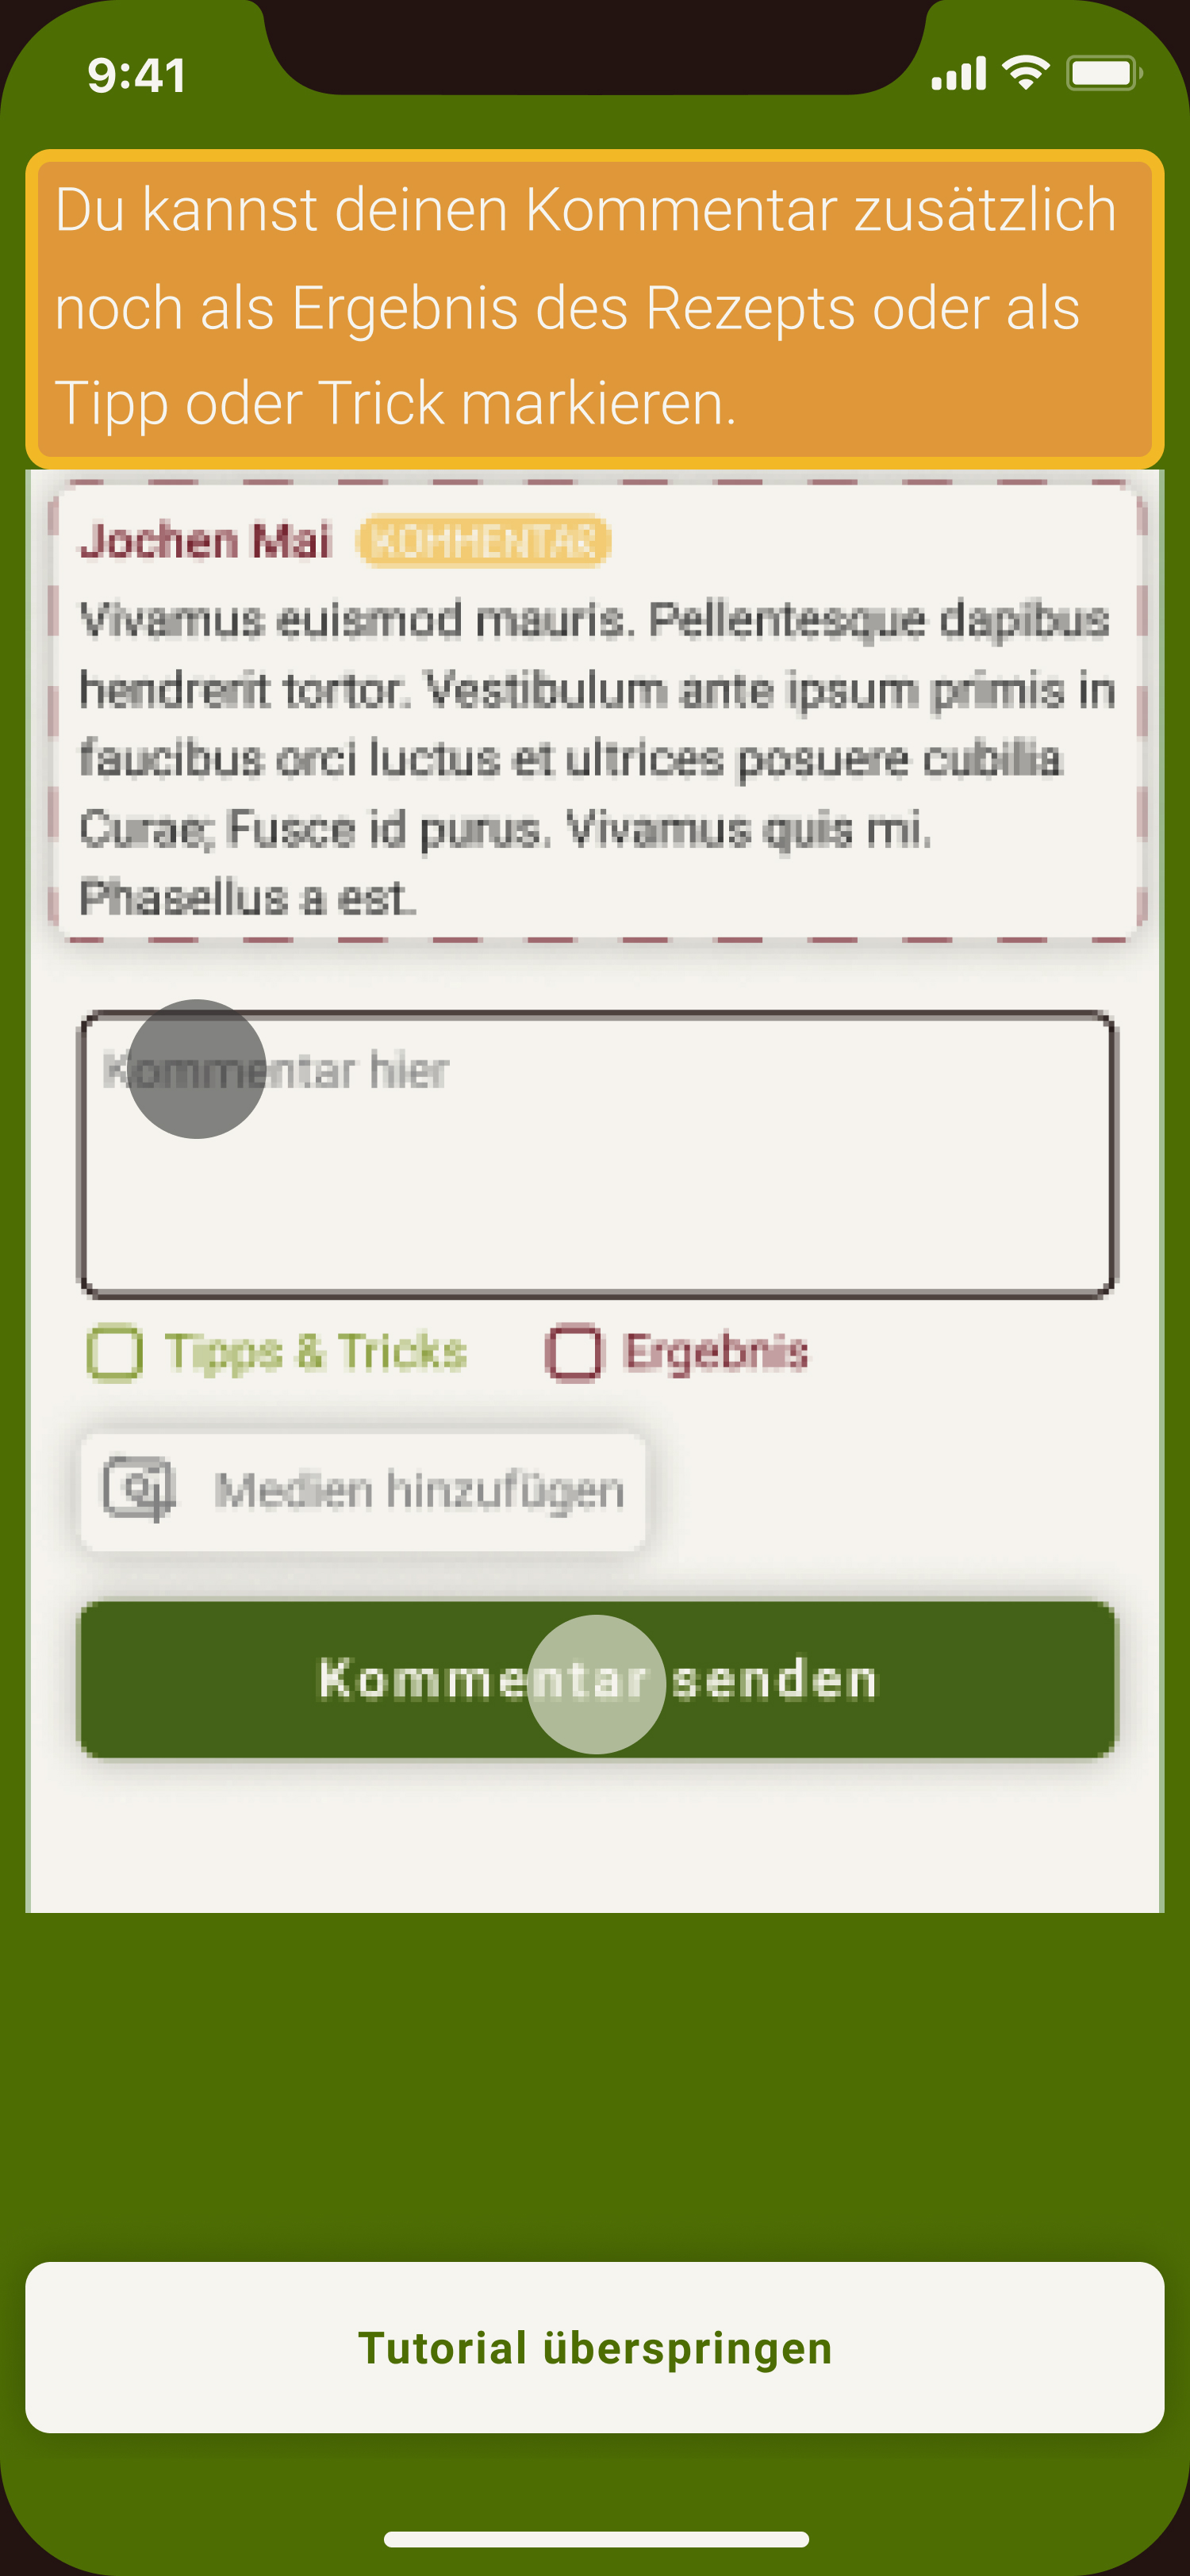
\includegraphics[width=0.14\textwidth]{images/introduction.jpg}
    \caption[Mock Up - Einführung]{Mock Up - Einführung}
\label{fig:mockup-introduction}
    \center
        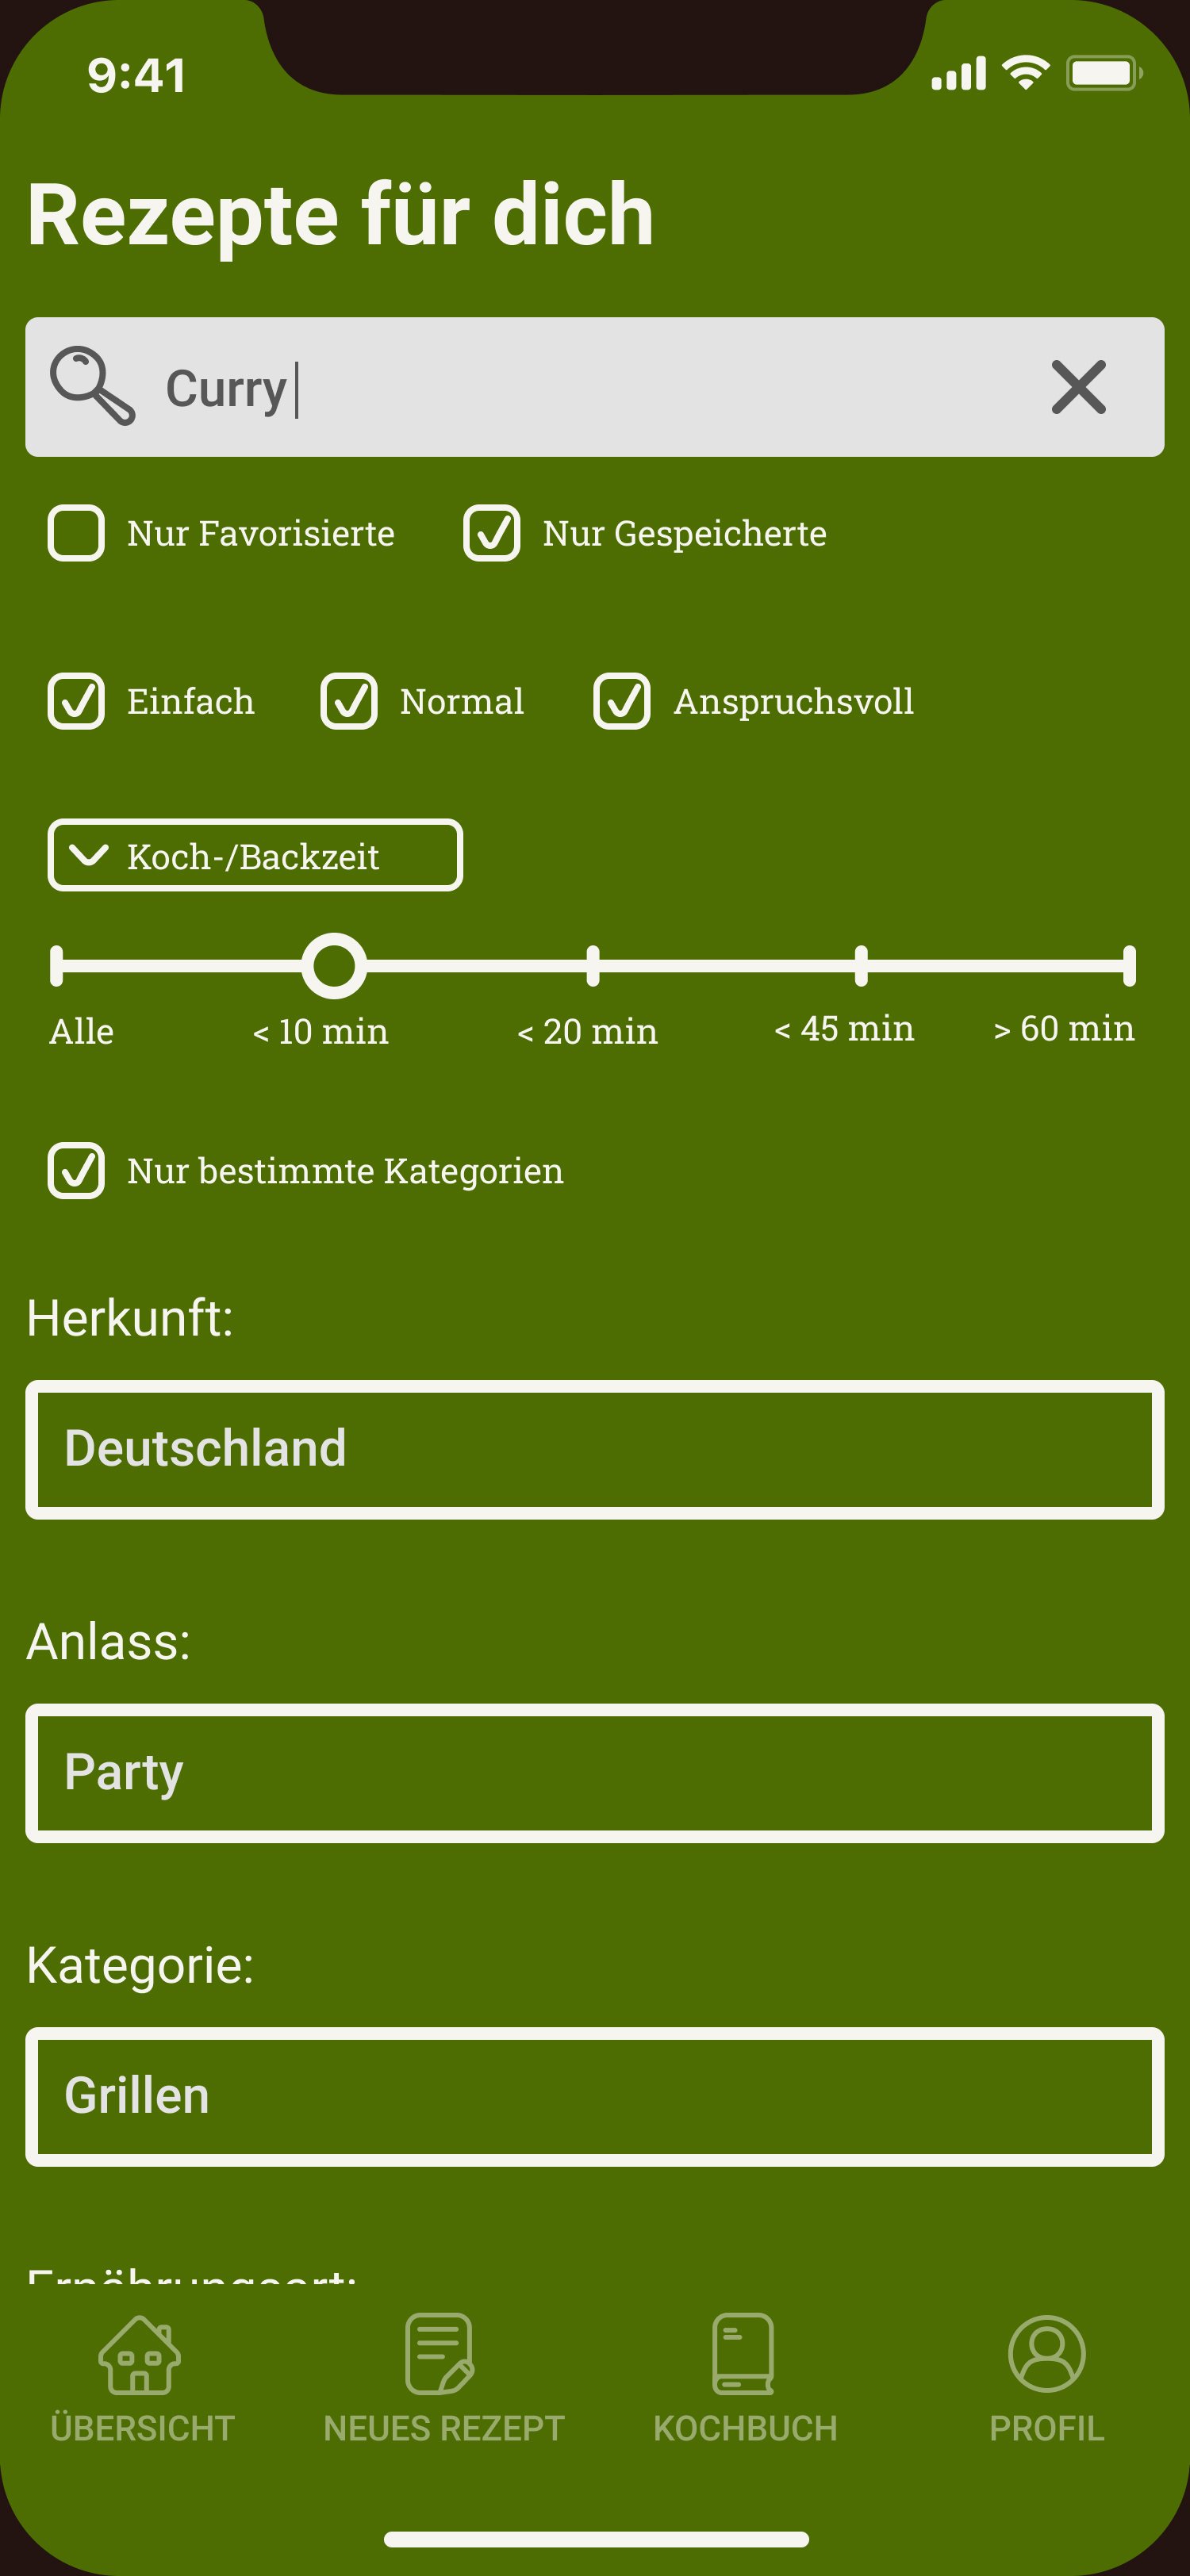
\includegraphics[width=0.14\textwidth]{images/filter.jpg}
    \caption[Mock Up - Filter]{Mock Up - Filter}
\label{fig:mockup-filter}
\end{wrapfigure}
Anhand der User Stories wurde entschieden, dass nach erfolgreichem Abschluss der Registrierung für den Dienst, im Sinne der Lernförderlichkeit, der Nutzer in das System eingeführt werden soll. Dabei werden die wichtigsten Funktionen mit Interaktiven Beispielen erklärt und mit Kommentaren erläutert. In dem Prototypen umfasst die Einführung das finden von Freunden und Familienmitgliedern über die Kontaktsuche, das Hinzufügen von Kommentaren zu Rezepten, wichtige Teile des Anlegens eines Rezepts, die nachträgliche Rezeptbearbeitung, das Suchen und Filtern von Rezepten und das Teilen von Rezepten mit Kontakten. \\
Um die Suche nach Rezepten die einen interessieren so intuitiv wie möglich zu gestalten, wurden anhand der User Stories Eigenschaften von Rezepten analysiert und diese dann durch gängige Praktiken in interaktive Filter implementiert. Ein Beispiel dafür ist der Filter nach Zubereitungsdauer. Hier wurden im wesentlichen die fünf durchschnittlich häufigsten Zubereitungsschritte gewählt und in einem simpel verständlichen Slider implementiert. Auch Checkboxen, um bestimmte Eigenschaften eines Rezeptes in den Sucheregbnissen zu inkludieren oder zu ignorieren, sind Resultate dieser Analyse. Für Meta-Eigenschaften, wie die Herkunft eines Rezeptes, welche geringfügig mit der Zubereitung zu tun haben, wurde der Filter als Dropdown Menu mit automatischer Vervollständigung implementiert. Das soll die Nutzbarkeit erhöhen, aber auch wie der Filter selbst die Fehlertoleranz erhöhen, da hier nur die Eigenschaftsdaten eingegeben werden können, welche auch tatsächlich in den Rezeptdatensätzen vorkommen. \\

\begin{wrapfigure}{r}{0.38\textwidth}
    \centering
        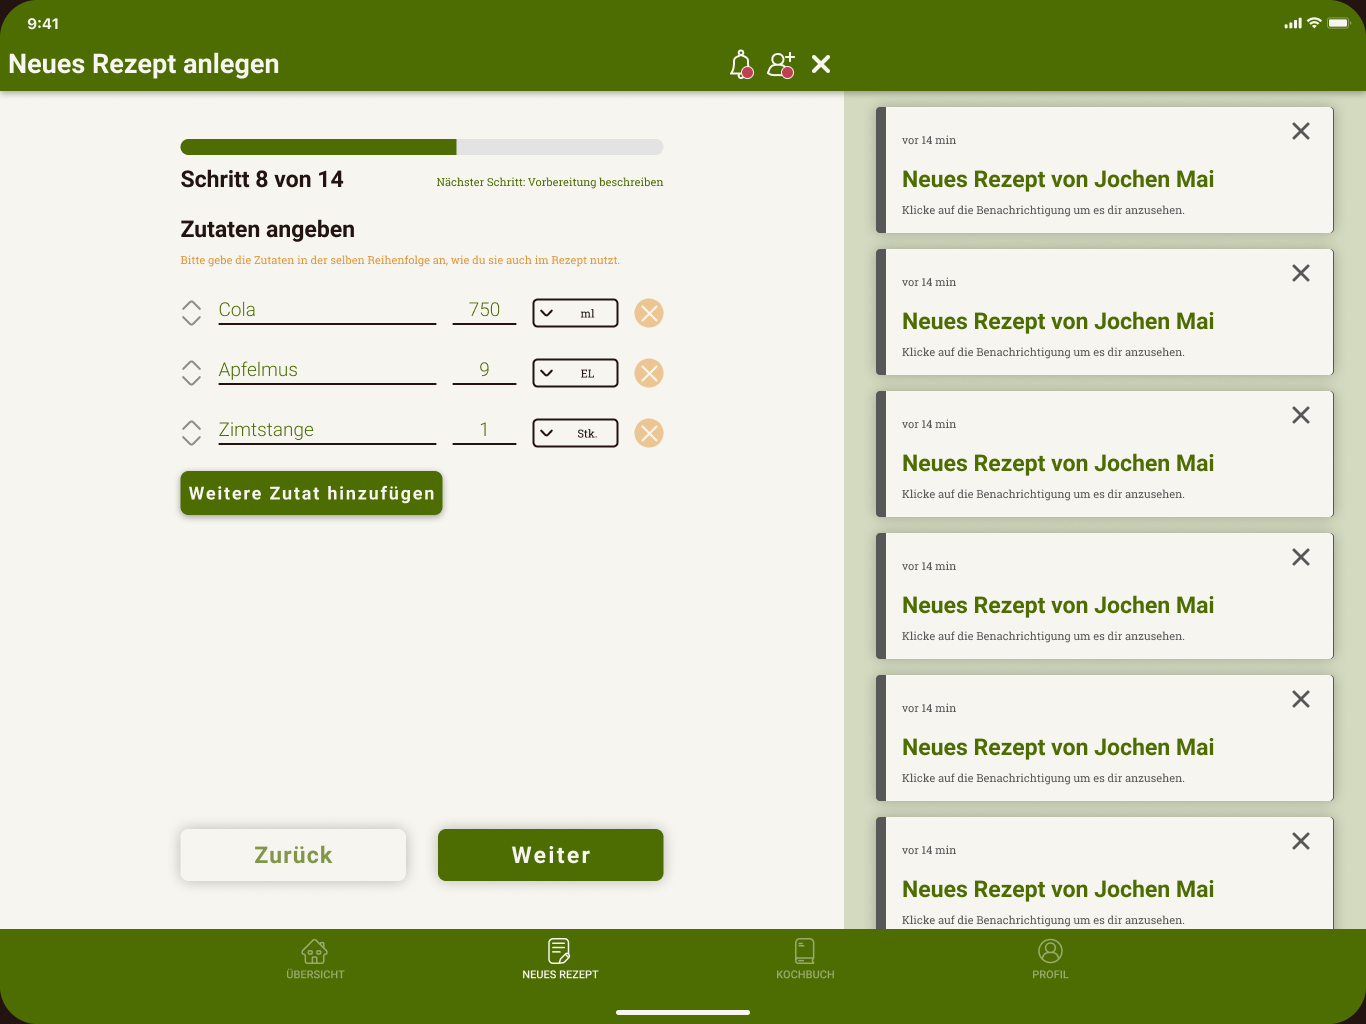
\includegraphics[width=0.38\textwidth]{images/addingredient.png}
    \caption[Mock Up - Zutaten angeben]{Mock Up - Zutaten angeben}
\label{fig:mockup-addingredient}
    \centering
        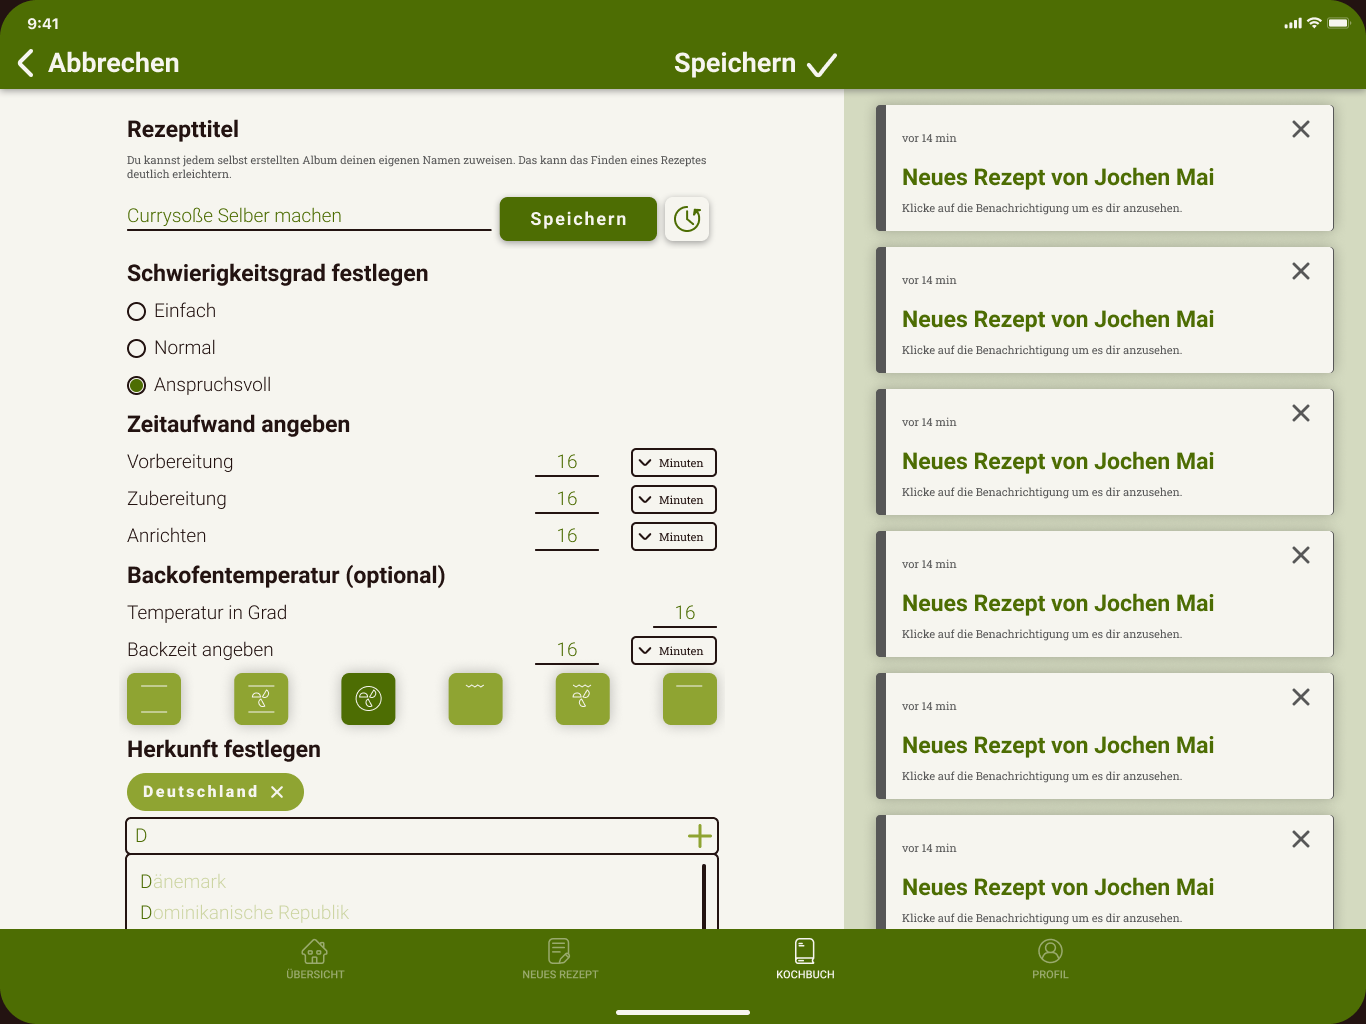
\includegraphics[width=0.38\textwidth]{images/editrecipe.png}
    \caption[Mock Up - Rezept bearbeiten]{Mock Up - Rezept bearbeiten}
\label{fig:mockup-editrecipe}
    \centering
        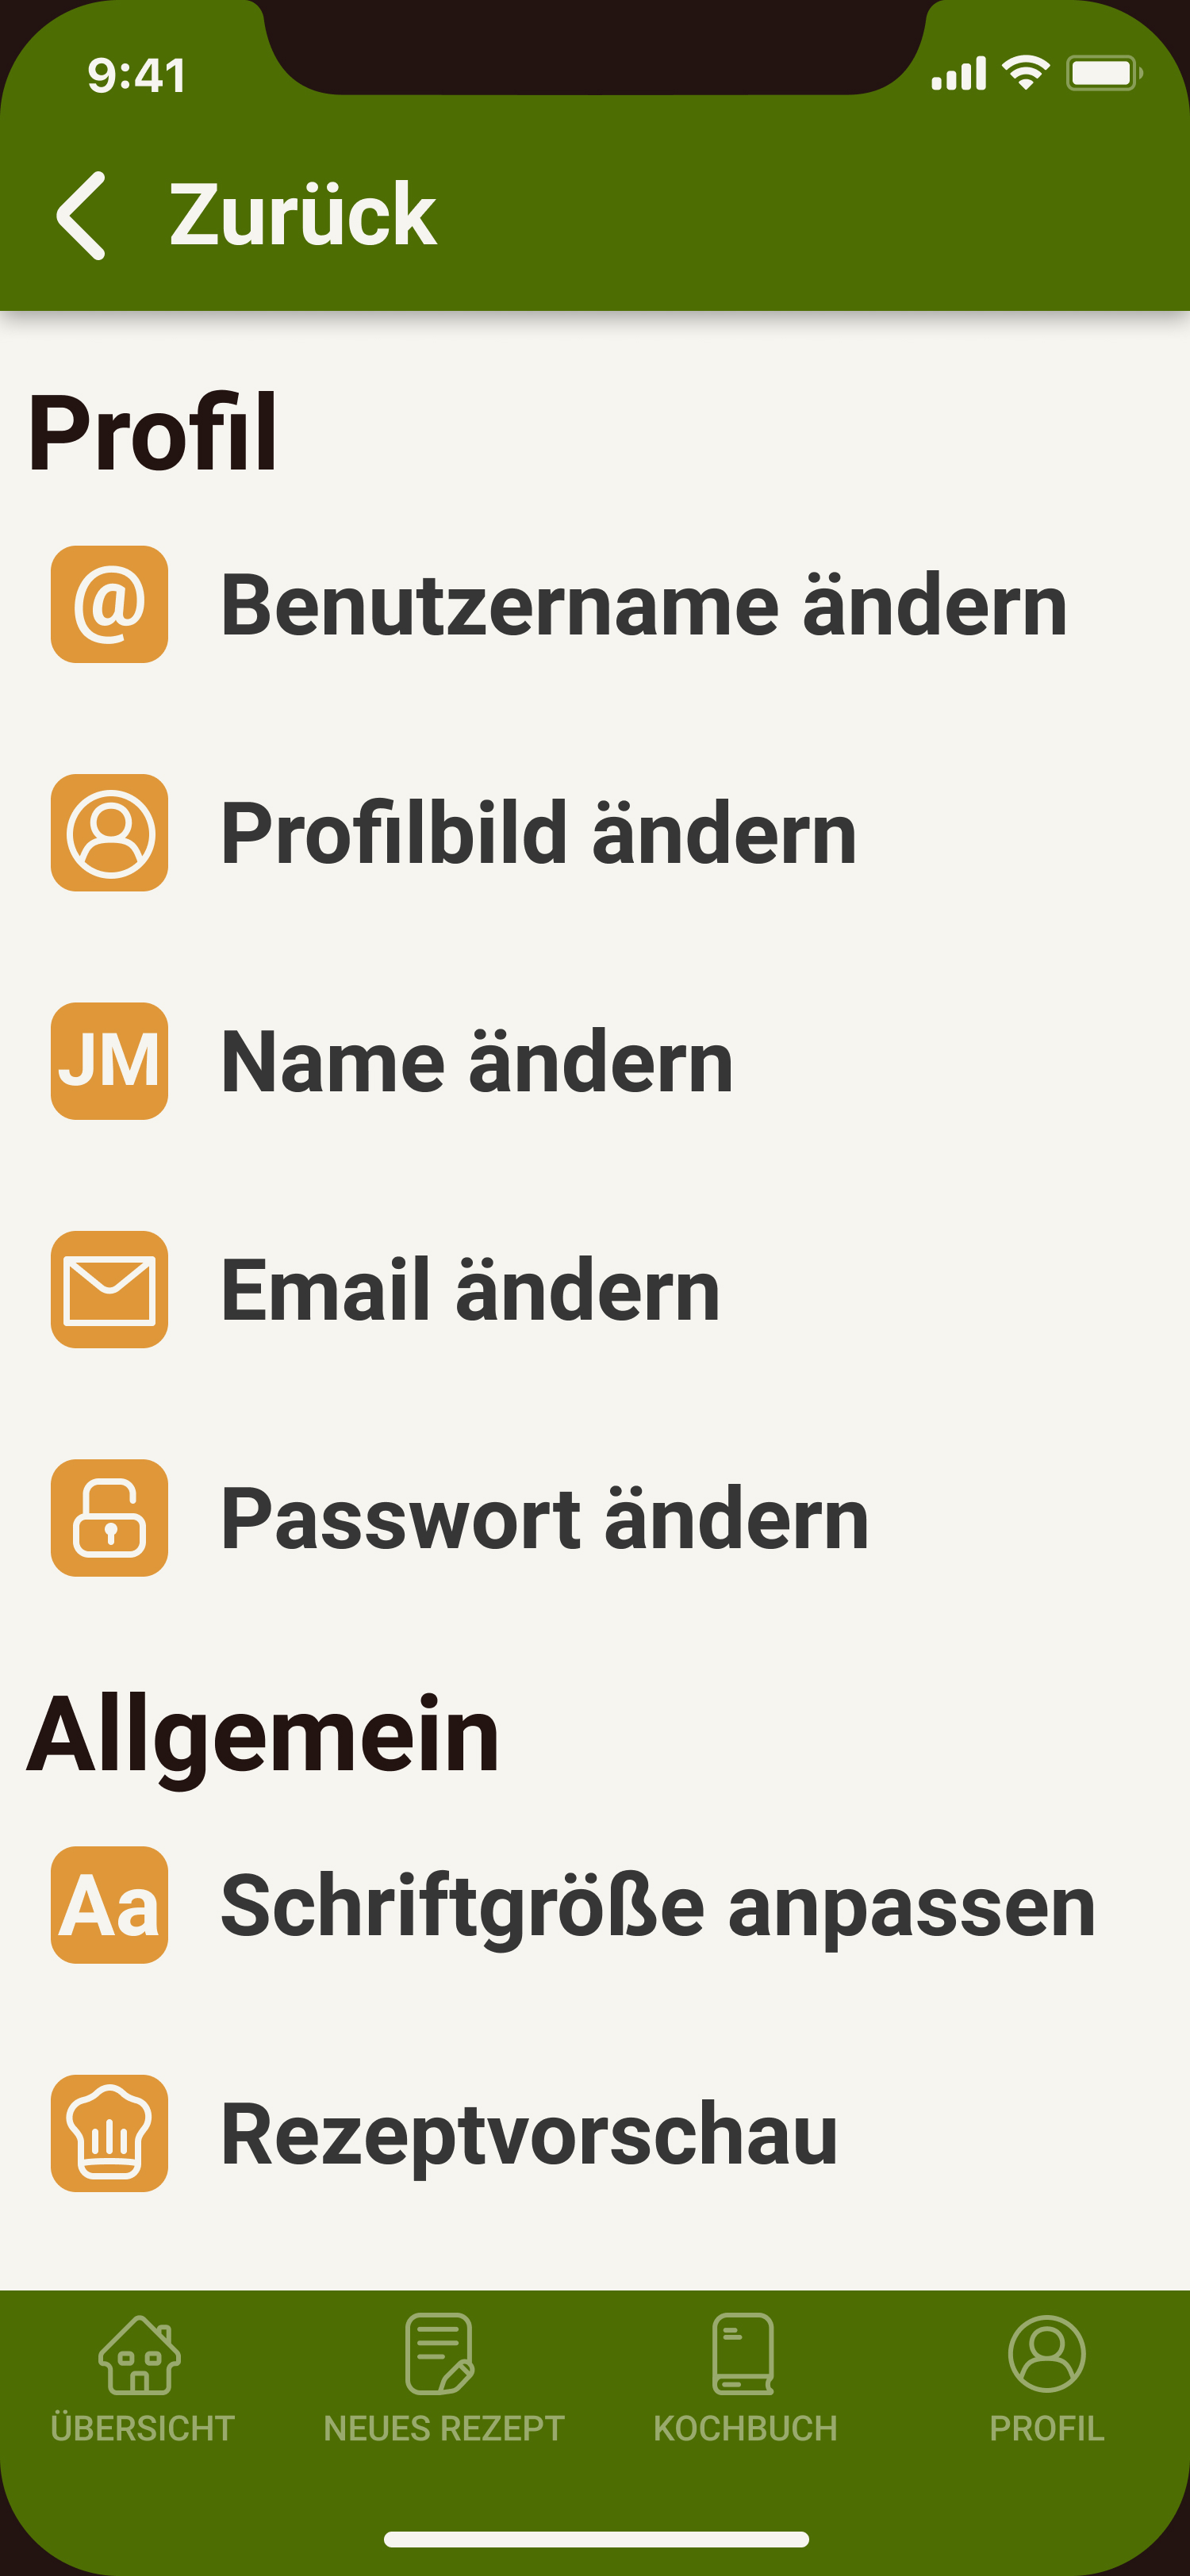
\includegraphics[width=0.14\textwidth]{images/settings.jpg}
    \caption[Mock Up - Einstellungen]{Mock Up - Einstellungen}
\label{fig:mockup-settings}
\end{wrapfigure}
Damit der Benutzer über Änderungen des Zustandes des interaktiven Systems informiert werden kann wurde eine Progressbar implementiert die sich am Kopf der Seite für das anlegen eines Rezeptes befindet. Um den Bildschirm nicht zu überladen wurden zusätzliche Informationen wie der Name des nächsten Schritts ausgeblendet. Für Desktop und Tablet Bildschirme ist diese Information verfügbar. \\
 Im Sinne der Steuerbarkeit wurden die Buttons ähnlich wie bei dem Blättern einer Seite in einem Buch am unteren Bildschirmrand platziert und durch klare visuelle Unterschiede hierarchisiert. So ist der Button für das fortsetzten der Bearbeitung mit der primären Farbe unterlegt und der Button für zurück farblich inversiert, was auch auch die invertierte Funktionalität wiedergibt. Der Button für das Überspringen eines Schrittes ist nur dann eingblendet, wenn ein Schritt für die Funktionalität des Kochbuchs nicht von belang ist. Der Button wurde somit nach dem Styleguide auch mit der Variante für die geringste Bedeutsamkeit ausgewählt um den Nutzern diese Funktion zwar anzubieten aber nicht als bevorzugt vorzulegen. \\
Für das Mock Up aus Abbildung \ref{fig:mockup-editrecipe} wurde entschieden, dass wenn Nutzer ein Rezept bearbeiten wollen, sie das gesamte Rezept editieren müssen. In der späteren technischen Umsetzung soll es dann noch die Möglichkeit geben an eine gewisse Stelle in der Rezept bearbeitung zu springen um ein ähnliches Verhalten wie das edititeren einzelner Komponenten herzustellen. Für aussreichende Ergonomik sorgen die bereits bekannten Eingabevarianten der Rezepterstellung und die praktisch plazierten Steuerbuttons in der Titelleiste für das Abbrechen oder Speichern der bisher getätigten Änderungen an dem Rezept. \\
Ein intuitver Einstellungsscreen der die Einstellungen eines Smartphones imitiert bietet nicht nur die Konfigurationsmöglichkeit für Benachrichtigungen, Profil und Datenschutz, sondern auch für Schriftgröße und Akzentfarben des eigenen Kochbuchs und des gesamten Systems. Um das System nicht unbrauchbar durch Nutzeranpassungen lassen zu werden, sind die Auswahlmöglichkeiten dennoch auf realisitische Alternativen beschränkt mit Ausnahme der Akzentfarbe welche über HexCodes oder einen ColorPicker verändert werden können. Diese Anpassungen sind ganz und gar der Individualiserbarkeit verschrieben. \\
% Lernförderlichkeit, Steuerbarkeit, (Fehlertoleranz), Individualisierbarkeit
% die anfänglichen Gestaltungslösungen befriedigen selten sämtliche Erfordernisse der Benutzer;
% Analysieren der Ergebnisse, Festlegen von Schwerpunktthemen und Unterbreiten von Lösungsvorschlägen;

\subsubsection{Prototypen}
Die Erarbeitung der Prototypen verlief nach dem Mobile First Prinzip. Dabei wird zuerst das Mobile Design erarbeitet um mögliche Probleme bei der Runterskalierung vorzubeugen. Tatsächlich hatte es den gegenteiligen Effekt. Da der bereits abgenommene Mobile Prototyp überarbeitet werden musste, nachdem es zu Problemen bei der Tablet Variante kam. Hier wurde das Designkonzept der Karten komplett überarbeitet und ihnen deutlich mehr Platz eingeräumt aber dafür auch mehr Weißraum gegeben, was wiederum für ein nutzerfreundlicheres und aufgeräumtes Interface sorgen soll. Insgesamt wurde die Prototypen für alle in den Userstories enthaltenen Screens erarbeitet und umfassen die Endgeräte Mobile (Iphone X), Tablet (Ipad Pro) und Desktop (MacBook Pro). Dabei handelt es sich nur um die Bildschirmgrößen und die Erweiterung um native UI Elemente um das Interface lebendiger wirken zu lassen. \\
Der Fokus des Systems liegt bei dem Mobilen Prototypen bei der Übersicht von Rezepten und Sozialen Interaktionen wie Kommentare zu verfassen und Freunde zu verwalten, da anzunehmen ist, dass Nutzer ihr Smartphone eher dafür nutzen auf dem aktuellen Stand zu bleiben oder sich mitzuteilen. Für den Tablet Prototypen liegt der Fokus auf der Übersichtlichkeit der einzelnen Rezepte in der Detailansicht, um sie in der Küche leichter kochen zu können. Dabei können Rezepte im Portrait Modus angesehen werden für mehr Screenestate. Für den Desktop Prototypen liegt der Fokus auf den Such- und Verwaltungsmethoden von Rezepten. So ist der Filter auf der rechten Sidebar sichtbar und die Suchergebnis links in Kartenform. Somit hat der Nutzer die Möglichkeit alle wichtigen Filteroptionen zu jedem Zeitpunkt einzusehen und zu modifizieren. \\
Das Programm für die Erarbeitung und Evaluierung der Protypen ist Figma, da es die Möglichkeit bietet, die Mockups um Interaktionen zu erweitern und dann auch interaktiv zu durchklicken. \\
\begin{figure}[h] %!=overrides latex; h=here; t=top; b=bottom; p=special page for floating objects
    \center
    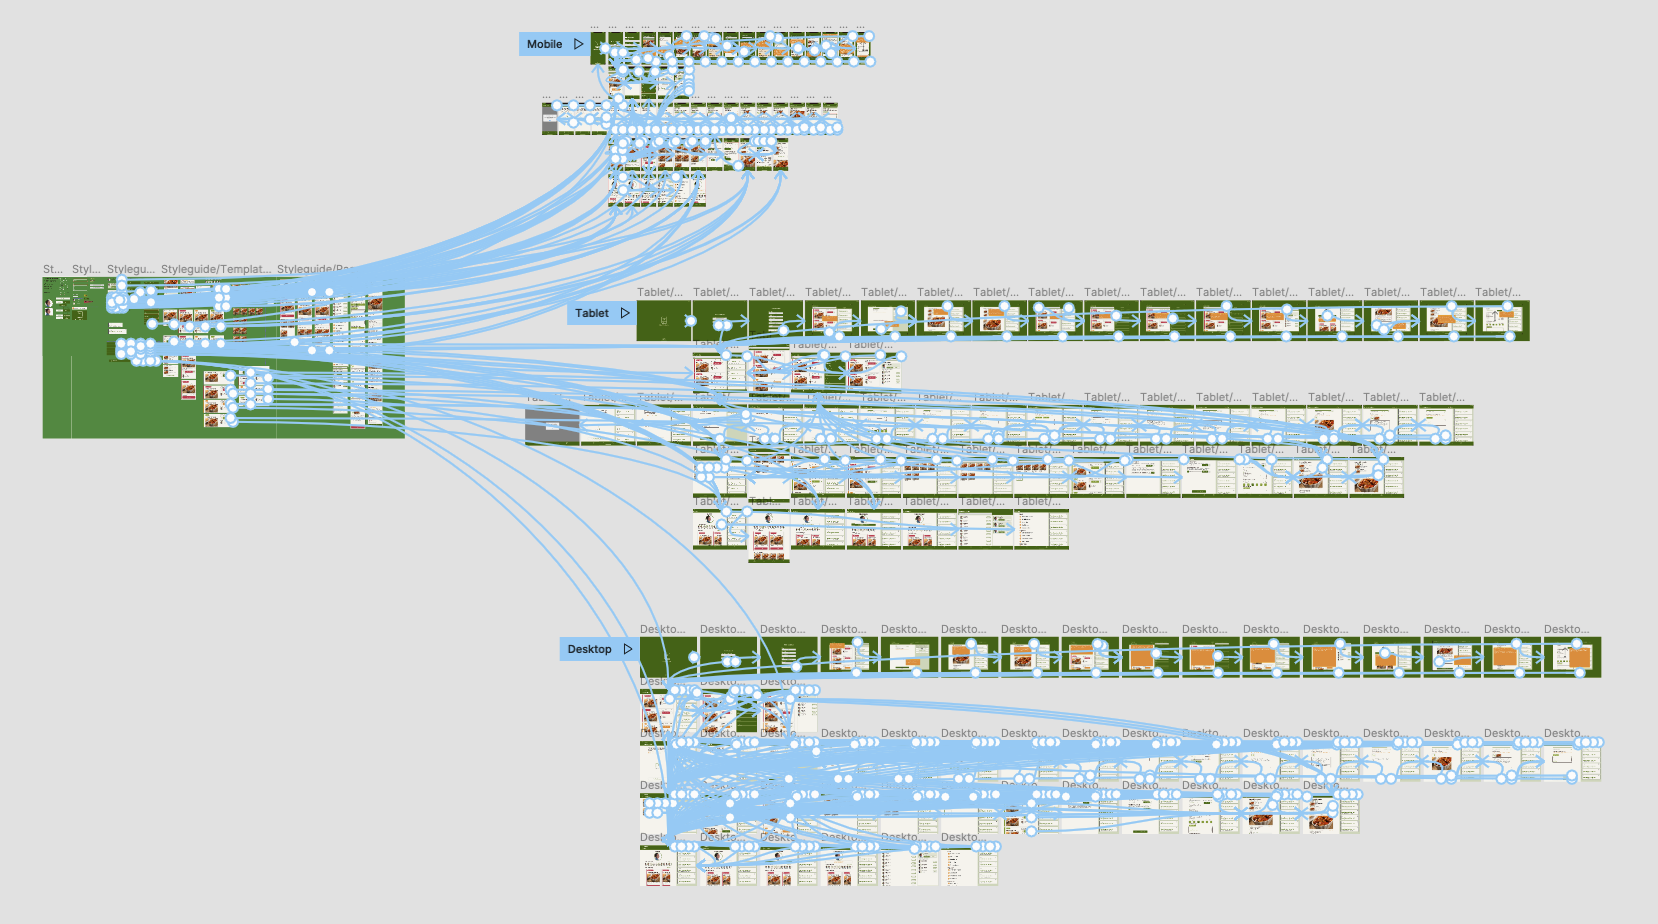
\includegraphics[width=0.8\textwidth]{images/prototyping.png}
    \caption[Prototypen in Figma]{Prototypen in Figma}
    \label{fig:prototyping}
\end{figure}

\subsection{Software Architektur}
Ausgehend von den User Stories aus \ref{sec:userstories}, lassen sich technische, aber Technologie unabhängige Anforderungen an das System ermitteln. 

\subsubsection{Minimal Viable Product}
\begin{figure}[h] %!=overrides latex; h=here; t=top; b=bottom; p=special page for floating objects
    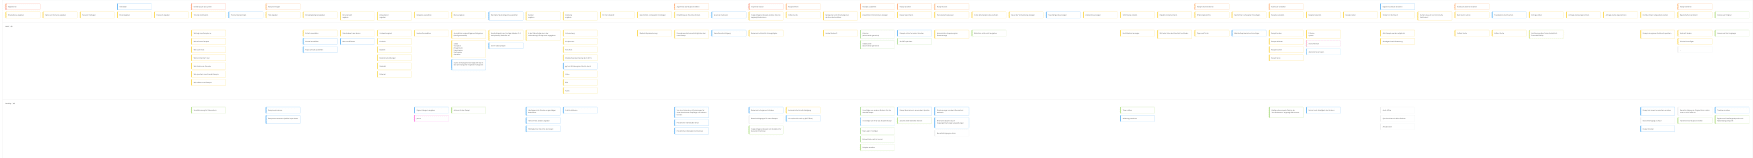
\includegraphics[width=1\textwidth]{images/mvp.png}
    \caption[Minimal Viable Product]{Minimal Viable Product}
    \label{fig:mvp}
\end{figure}
Während des Workshops wurden manche User Stories als zwingend notwendig identifiziert und bildeten so das Rückgrat des Storyboards. Mit fortlaufender Dauer des Workshops wurden Funktionen und Schritte an den verschiedenen Stellen ergänzt, wo durch teilweise sehr hohe Stacks entstanden. Um diese User Stories in den MVP zu überführen wurden die User Stories priorisiert und in Now und Not Now aufgeteilt. Hier kam es zu längeren Diskussionen, da die Teilnehmer nicht immer einer Meinung waren. Das Ergebnis des Workshops bildet jedoch einen von allen Teilnehmern akzeptierten Kompromiss ab. Im Nachgang an den Workshop wurden diese Erwartungen und Erfordernisse in Anforderungen an das System und dessen Architektur überführt.\\

\subsubsection{Abhängigkeiten der Anforderungen}
\begin{wrapfigure}{r}{0.38\textwidth}
    \centering
    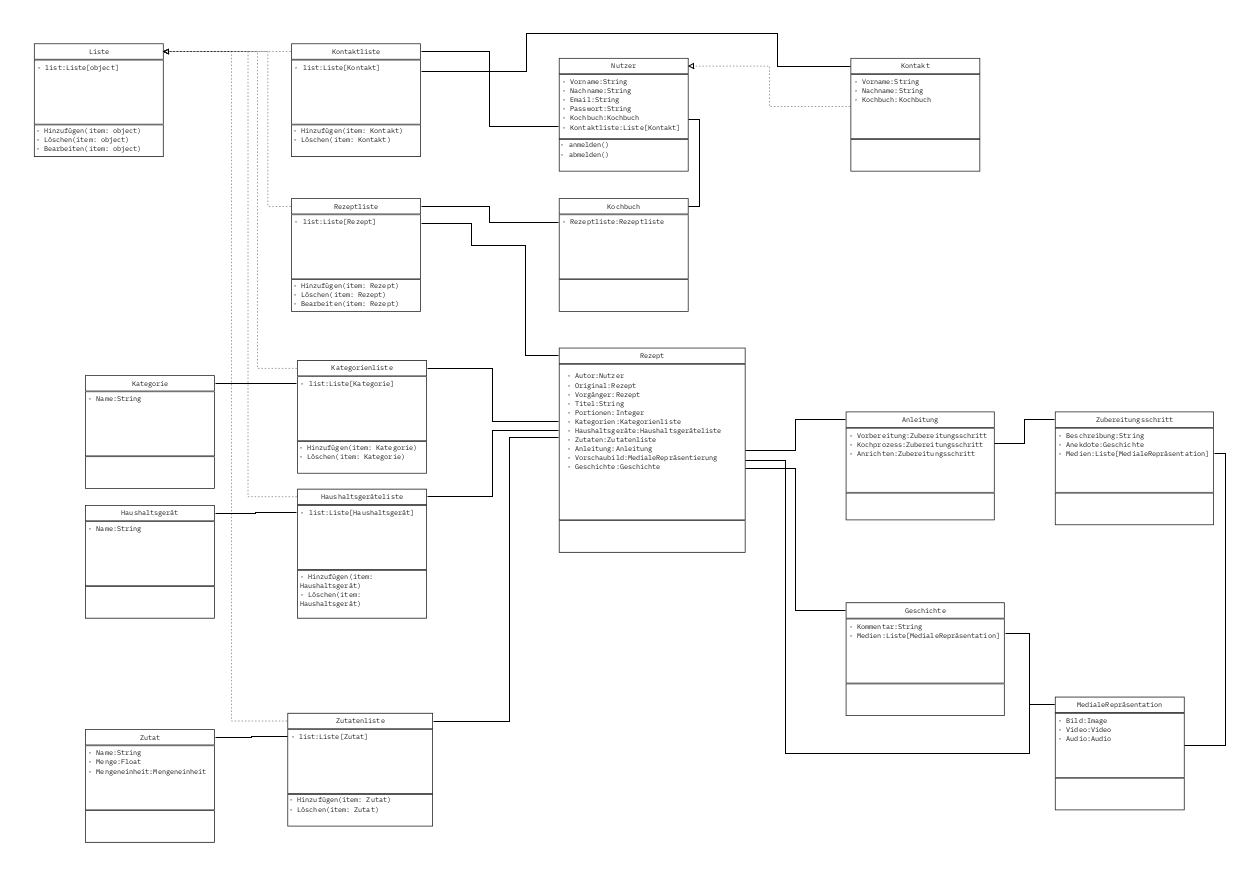
\includegraphics[width=0.35\textwidth]{images/dependencymodell.png}
    \caption[Abhängigkeitsmodell]{Abhängigkeitsmodell}
    \label{fig:dependencymodell}
\end{wrapfigure}
Die Anforderungen an das System wurden auf Abhängigkeiten untersucht und Lösungen für diese Abhängigkeiten oder daraus resultierende Folgen für das System notiert. In der Abbildung \ref{fig:dependencymodell} sind die Abhängigkeiten zwischen den zu speichernden Daten visualisiert. Um die gesammelten Lösungsansätze für die Abhängigkeiten weiter einzugrenzen wurden hypothetische Lösungen in einer Umfrage an die Nutzer vorgestellt. Das Ergebnis der Umfrage hat die System Architektur maßgeblich geprägt.\\

\subsubsection{Systemarchitektur}
\begin{figure}[h] %!=overrides latex; h=here; t=top; b=bottom; p=special page for floating objects
    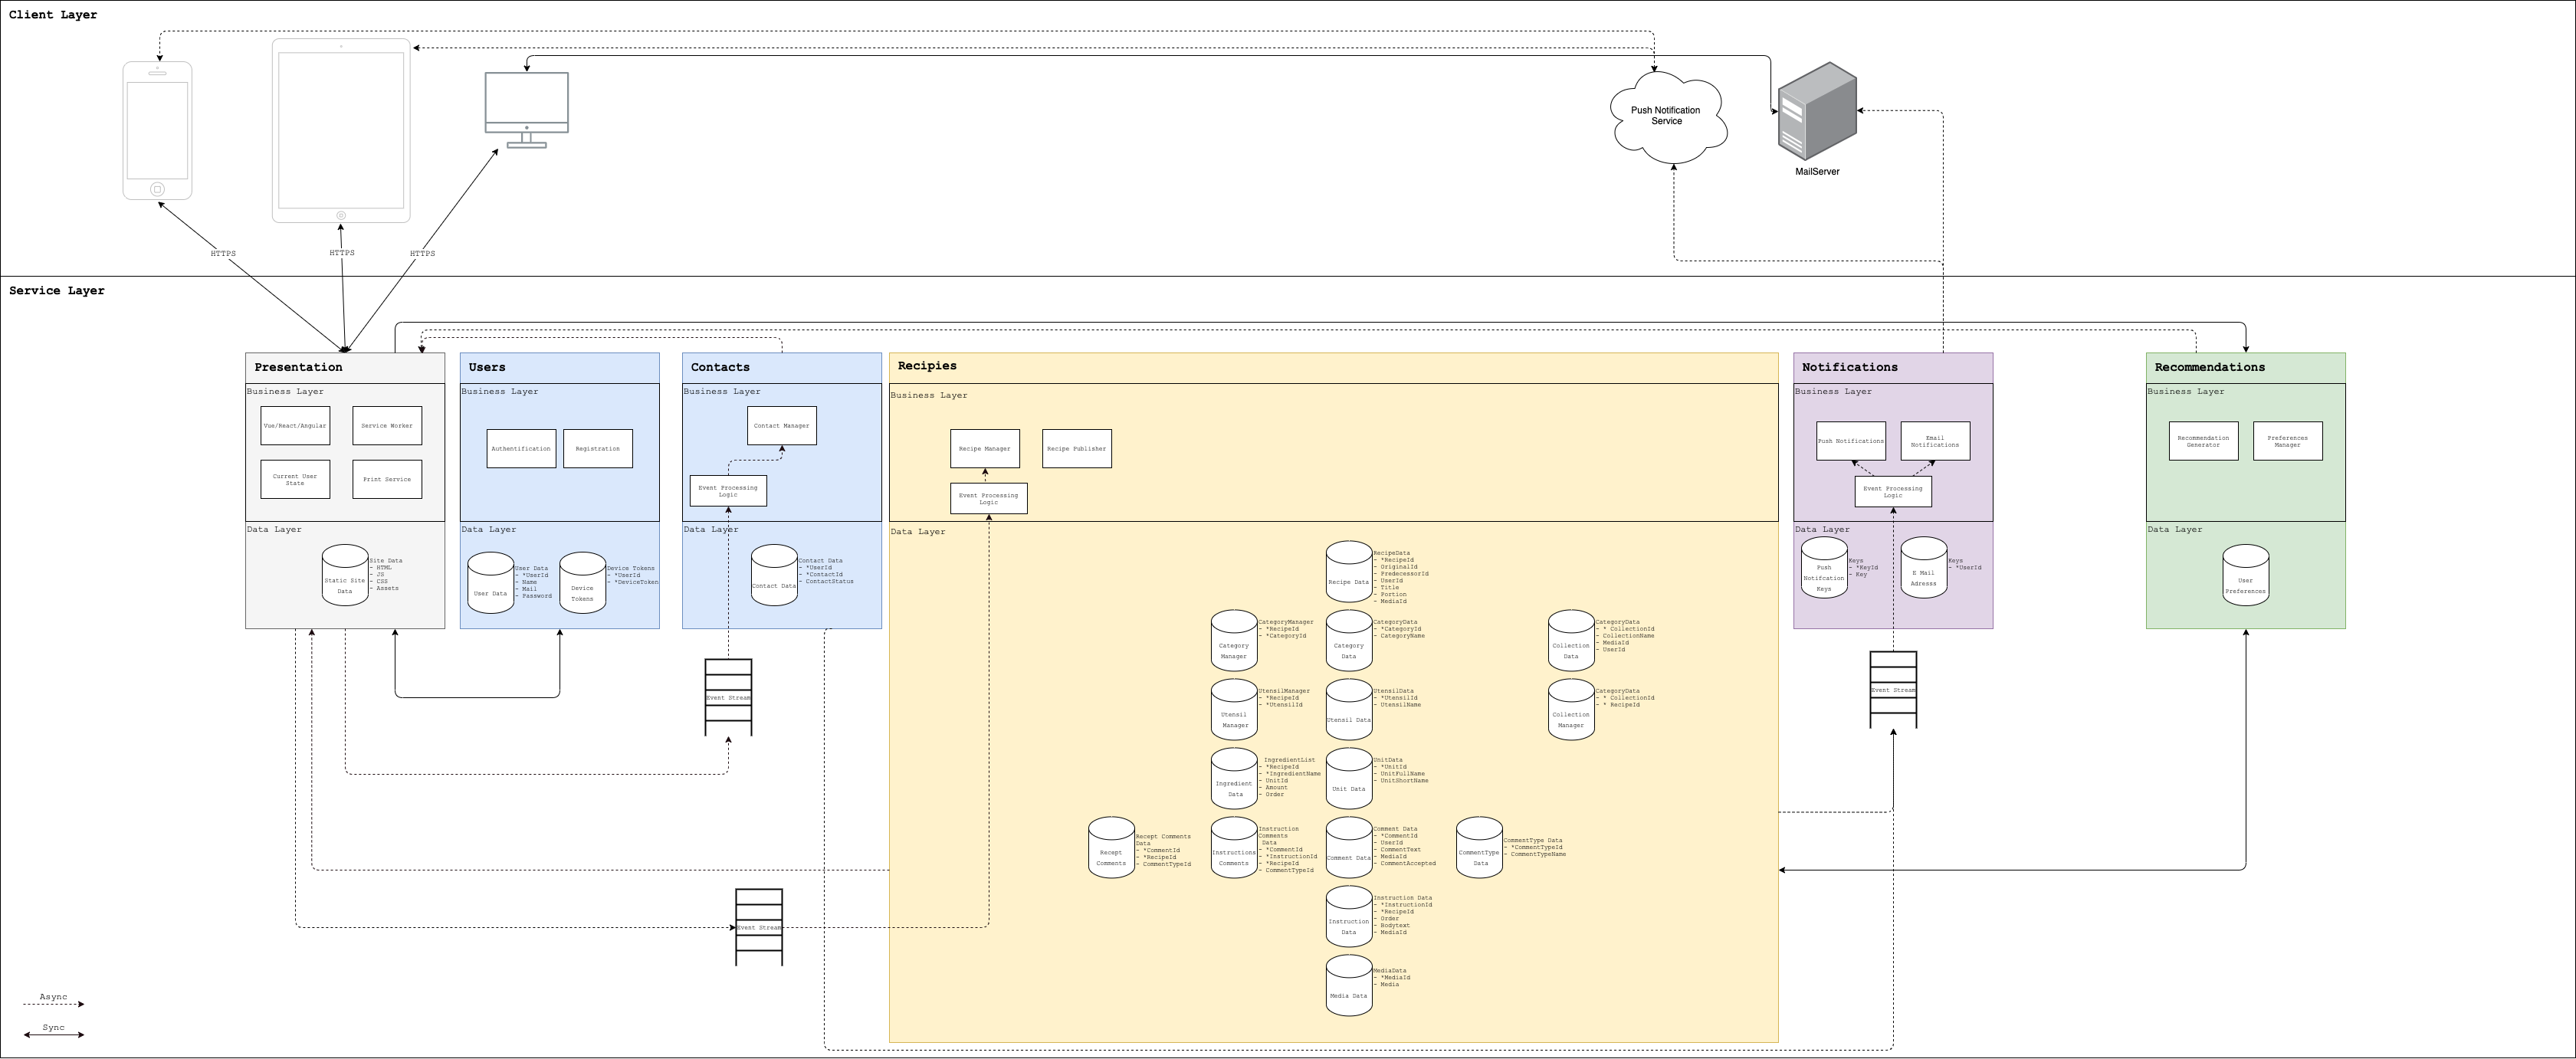
\includegraphics[width=1\textwidth]{images/systemarchitechure.png}
    \caption[Systemarchitektur]{Systemarchitektur}
    \label{fig:systemarchitechure}
\end{figure}
Das System wird auf zwei Ebenen liegen. Eine Ebene ist die Client Ebene. Hier wird die Anwendung auf den jeweiligen Endgeräten laufen und Benachrichtigungen empfangen. Die Service Ebene besteht aus 6 Service Komponenten welche jeweils eine bestimmte Aufgabe des Systems übernehmen. Diese Aufteilung soll das System skalierbarer machen und ebenfalls die Wartbarkeit fördern. Der Präsentationsservice stellt das Frontend über HTTPS den Endgeräten zur Verfügung und wird wahrscheinlich in JavaScript Frameworks wie Vue, Angular oder React implementiert sein, da hier die Möglichkeit gegeben ist aus einer Progressiven Web Applikation eine Native App zu erzeugen, was wiederum die Erreichbarkeit des Systems vergrößern würde. Auch Funktionen wie die Druckfunktion, als der Transfer von einem Rezept in HTML zu einem PDF zu exportieren und zu drucken, oder die Offline Funktion zum lesen von Rezepten ohne aktive Internetverbindung. Die Servicekomponenten für Clients und Kontakte verwalten die Lese und Schreibrechte für die Nutzer und sind daher essentiell für die Sicherheit des Systems. Für die Rezepte ist ein relationelles Datenbankschema angedacht welches die Rezepte in einzelne Tabellen aufteilt um auch hier den Abruf einzelner Informationen oder das aktualisieren von Rezeptbestandteilen zu erleichtern. Die Benachrichtigungskomponente verfügt über den Anschluss an einen Mailserver des Systems und an Push Notfication Services um Nutzer über neue Rezepte nach Bedarf zu benachrichtigen. Die Empfehlungskomponente generiert in regelmäßigen Abständen Daten die darüber Aufschluss geben sollen welcher Nutzer welche Rezepte seines Bekanntenkreises mögen könnte, um somit mit einer gewissen wahrscheinlichkeit ihn dazu zu bringen sich mit kulturell interessanten Rezepten zu beschäftigen. Die Komponenten sollen möglichst lose gekoppelt sein, bedürfen aber einiger Kommunikationsschnittstellen. Für die Kommunikation zwischen Client und Server ist eine REST Schnittstelle angedacht, innerhalb des Systems jedoch wird auf asynchrone Kommunikation über Nachrichten gesetzt. Das soll das System instand haltbarer, performanter und ausfallsicherer machen. \\
Zu bedenken ist jedoch, dass dieses Architekturmodell nur eine Lösung ist und sich gegebenenfalls während der Implementierung noch verändern könnte, auf Grund von der Änderung der Anforderungen oder der Nutzung effektiverer Technologien.
% einige Anforderungen zeigen sich erst dann, wenn ein Lösungsvorschlag vorliegt;
\subsubsection{Pseudocode}
Für die Anwendungslogik der ähnlichen Rezepte unter einem angesehenen Rezept, müssen zunächst Rezepte gekocht oder als gespeichert markiert werden. Als gekocht zählen Rezepte welche über den Button als gekocht markiert werden oder länger als 5 Minuten betrachtet worden sind. Als gespeichert gelten die Rezepte welche über den Button als gespeichert markiert wurden. Die Dauer die ein Nutzer ein Rezept betrachten muss um es automatisch als gekocht zu markieren ist nicht festgeschrieben und wird gegebenenfalls durch die Auswertung des MVPs angepasst. \\
Das aktuell betrachtete Rezept wird ausgewertet und dessen als relevant betrachteten Attribute gesammelt. Für jedes markierte Rezept werden ebenfalls die relevanten Attribute gesammelt. Doppelt vorkommende Rezepte werden reduziert. Darauf hin werden alle markierten Rezepte durchlaufen und die Häufigkeit der vorkommenden Attribute hochgezählt. Daraus ergeben sich dann die Präferenzen des Nutzers. Als Nächstes wird jedes Rezept, also gespeicherte und neue, unbekannte, durchlaufen und für jedes Attribut das im aktuell betrachteten Rezept ebenfalls vorkommt wird der Score des Rezept erhöht. Für jedes Attribut, dass auch in den Präferenzen mit besonders hohem Vorkommen enthalten ist, wird der Score des Rezept zusätzlich erhöht. Anschließend wird der Score des Rezepts durch die Anzahl seiner Attribute geteilt. Die Liste der Rezepte wird nach dem Score absteigend sortiert und dann die ersten fünf Ergebnisse zurückgegeben. \\
\begin{lstlisting}[caption=Pseudocode - Ähnliche Rezepte,label={lst:SimilarRecipies}]
// Mark Recipe as cooked
if (thisRecipe.isOpen() > 300000) { // Opened for longer than 5 minutes
    if(!MY.cookedRecipes.contains(thisRecipe)) { 
        MY.cookedRecipes.add(thisRecipe);
    }
}

button[cookThis].isPressed() => {
   if(!MY.cookedRecipes.contains(thisRecipe)) {
        MY.cookedRecipes.add(thisRecipe);
    }
}

// Save Recipe
button[saveThis].isPressed() => {
   if(!MY.savedRecipes.contains(thisRecipe)) {
        MY.savedRecipes.add(thisRecipe);
    }
}

// Get MetaData from this Recipe
JSON thisRecipeMetaData = thisRecipe.getMetaData();

// Get Saved Recipe Preferences
JSON savedRecipePreferences = MY.getSavedRecipePreferences();

// Get Cooked Recipe Preferences
JSON cookedRecipePreferences = MY.getCookedRecipePreferences();

// Get similar Recipes
function getSimilarRecipes(currentRecipeMetaData, savedRecipePrefs, cookedRecipePrefs) {
    var searchForPrefsLikeThis;
    searchForPrefsLikeThis.addWithBasicImportance(currentRecipeMetaData);

    comparePrefWithMeta(savedRecipePrefs, currentRecipeMetaData)
    comparePrefWithMeta(cookedRecipePrefs, currentRecipeMetaData)
    
    function comparePrefWithMeta(prefs, meta) {
        for each Attribute in Pref {
            if meta[Attribute] == Pref[Attribute] {
                if(searchForPrefsLikeThis.contains(Attribute)]) {
                    searchForPrefsLikeThis[Attribute].increaseImportance();
                } else {
                    // Do Nothing
                }
            }
        }
    }

    var similareRecipes = OurServer.makeSearch(searchForPrefsLikeThis);

    return similarRecipes
}

// Make Search on our Server Side
function makeSearch (parameters, user) {
    var result;

    var params = parameters;

    var user = user;
    var friends = user.getFriendIDs();
    
    var userRecipes = user.getRecipeIDs();
    var friendRecipes;
    for each friend in friends {
        friendRecipes += friend.getRecipeIDs()
    }

    var allRecipeIDs = removeDuplicates(merge(friendRecipes, userRecipes));

    for each recipe in allRecipeIDs {
        var compareResult = recipe.compareWithParams(params);

        if(compareResult > 0.5) {
            result.add(recipe, compareResult)
        }
    }

    function compareWithParams (params) {
        var recipedata = this.getMetaData();
        var compareResult = 0;
        var attributesLength = recipedata.countAttributes();
        var score = 0;

        foreach Attribute in recipedata {
            if recipedata[Attribute] == params[Attribute] {
                score++;
                if(params[Attribute].importance > 3) {
                    score++;
                }
            }
        }

        compareResult = score / attributesLength;
        return (double) compareResult;
    }

    result.sortBy(compareResult);               
    //Sort all results by their rating
    result.stripAllButFiveStartingAtFirst();    
    //Remove all but the 5 first in List

    return result;
}
\end{lstlisting}
Für die Empfehlung von Rezepten auf der Startseite soll basierend auf der lokalen Zeit alle Menüs und Saisons gesammelt werden um diese dann zusammen mit dem Präferenzen des Nutzers in einer Abfrage zu bündeln. Dabei werden von allen verfügbaren Rezepten alle die nicht das Menü oder nicht in der Saison enthalten sind aus der Ergebnismenge entnommen. Anschließend werden Rezepte die die Saison oder das Menü als Attribute enthalten in ihrer Wichtigkeit erhöht. Das soll Rezepte die weder ein Menü noch eine Saison gepflegt haben, in ihrer Wichtigkeit reduzieren, da sie bei der ersten Reduzierung der Ergebnismenge nicht entfernt wurden. Anschließend werden wie oben die persönlichen Präferenzen des Nutzers auf die übrig gebliebenen Rezepte angewendet und die fünf Rezepte, wie auch schon in dem Pseudocode Ausschnitt \ref{lst:SimilarRecipies}, zurückerhalten und ausgegeben. \\
\begin{lstlisting}[caption=Pseudocode - Empfehlungen,label={lst:Recommendations}]
// Get Local Time
import Date from Libary;

function getLocalTime() {
    return Date.currentTime();
}

// Get Menu Based On Time
function getMenuBasedOnTime(localTime) {
    allMenus = OurServer.getAllMenus();

    foreach (allMenus as menu) {
        if (!isContainedIn(menu.typicalTimeRange, localTime)){
            allMenus.remove(menu);
        }
    }
} 
/* Probably easier to just return the prefered menu by the server time. We will do that, but for the sake of explaining the code, we stick with this */

// Get Season Based On Time
function getSeasonBasedOnTime(localTime) {
    allSeasons = OurServer.getAllSeasons();

    foreach (allSeasons as season) {
        if (!isContainedIn(season.typicalTimeRange, localTime)){
            allMenus.remove(season);
        }
    }
} 
/* Probably easier to just return the prefered season by the server time. We will do that, but for the sake of explaining the code, we stick with this */

// Get Saved Recipe Preferences
JSON savedRecipePreferences = MY.getSavedRecipePreferences();

// Get Cooked Recipe Preferences
JSON cookedRecipePreferences = MY.getCookedRecipePreferences();

// Get Recommendations
function getRecommendations(allMenus, allSeasons, savedRecipePreferences, cookedRecipePreferences) {
    var preferences = merge(savedRecipePreferences, cookedRecipePreferences);
    preferences.removeAllMenusBut(allMenus);
    preferences.removeAllSeasonsBut(allSeasons);
    preferences.boostImportanceOfSeasonAndMenu(); 
    //Increases Importance of Seasons and Menus so the search will likely deliver more fitting recipes

    var recommendations = OurServer.makeSearch(preferences); 
    //See at PseudoCode Similiar Recipes

    return recommendations;
}
\end{lstlisting}
\section{Evaluierung der Gestaltungslösungen anhand der Anforderungen}
Für den letzten Schritt des Praxisprojekts sollen die Gestaltungslösungen evaluiert werden und eine Zustand erreichen, bei dem die potentiellen Nutzer des Systems zufrieden gestellt sind. \\

\subsection{Prüfung durch Benutzer}
% Qualitativ das Beste Ergebnis um die Frage zu beantworten
Für die Evaluierung gibt es verschiedene Vorgehensweisen. Im gesamten Projektverlauf wurden stets die einzelnen Artefakte von Benutzern evaluiert. Somit konnten diese wesentliche Bestandteile des interaktiven Systems beeinflussen. Die größte Beteiligung bestand bei der Auswahl der Schriftarten und textuellen Gestaltung eines gedruckten Rezepts. Hier sollten die Grundsteine für den zu entwickelnden Styleguide gelegt werden um eine Richtung für die Mock Ups vorzugeben. Aber auch hier gab es Meinungsverschiedenheiten zwischen den Nutzern. \\
\begin{figure}[h] %!=overrides latex; h=here; t=top; b=bottom; p=special page for floating objects
    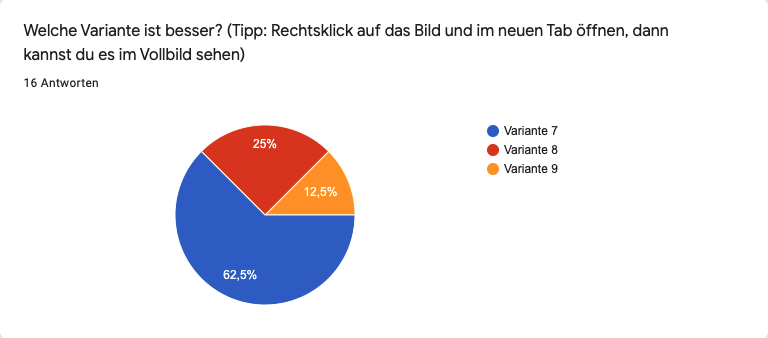
\includegraphics[width=1\textwidth]{images/EvaluierungBeispiel.png}
    \caption[Evaluierung - Beispiel]{Evaluierung - Beispiel}
    \label{fig:EvaluierungBeispiel}
\end{figure}
Im Nachgang an die durchgeführten Benutzerumfragen wurde nach dem höchsten Prozentsatz die Variante weiterentwickelt bis die Gestaltungslösung die größte Mehrheit erreichte. Während der Entwicklung der Mock Ups wurde eine wesentliche Anpassung der Karten ebenfalls anhand von Benutzerumfragen evaluiert und als die modernere, ergonomischere Lösung bewertet und folglich im gesamten Design umgesetzt. 

\subsection{Zeitliche Abstimmung und Ressourcen}
Im Rahmen des Praxisprojekts wurde die empirische Datenerhebung nur in kleinem Rahmen durchgeführt. Für die Bachelorarbeit sind Evaluierungen mit größeren Nutzergruppen angesetzt. Konkret bedeutet das, dass jeweils pro Umfrage fünf bis dreißig Personen befragt worden sind oder an der Umfrage teilgenommen haben. Bedauerlich ist, dass die letzte Evaluierung deutlich weniger Beteiligung erfuhr, vermutlich auf Grund des ungünstigen Zeitpunkts um Weichnachten 2021 herum. Für kommende Projekte ist daher zu vermerken, dass in den Ferien im Sommer herum die größte aktive Nutzerbeteiligung zu vermerken war. Ebenfalls zu vermerken ist, dass das angeleitete Evaluieren eine bessere Methode darstellt als die explorative Evaluierung, da nicht von jedem Nutzer zu erwarten ist, dass dieser seine Aufgabe gewissenhaft und gründlich löst. Eine User Story hingegen in eine Reihe von Aufgaben zu übersetzen und diese möglicherweise auch unter Beobachtung lösen zu lassen und die dabei erhaltenen Erkenntnisse zu dokumentieren, stellt vermutlich die bessere Alternative dar. Mögliche Hilfestellung bei der Findung von Resourcen für die Evaluierung, stellen selbstverständlich Verteiler der Technischen Hochschule Köln, die Betreuer des Projekts als auch Verbindungen durch den Arbeitgeber dar. Jedoch wurden diese auf Grund von zeitlicher Knappheit nicht in Anspruch genommen. Die oben genannten Punkte sollen daher in der Evaluierung der Ergebnisse in kommenden Projekten, wie zum Beispiel der Bachelorarbeit beachtet und umgesetzt werden. \\

\subsection{Analysieren der Ergebnisse}
% Zufrieden mit Feature Requests
\begin{figure}[h] %!=overrides latex; h=here; t=top; b=bottom; p=special page for floating objects
    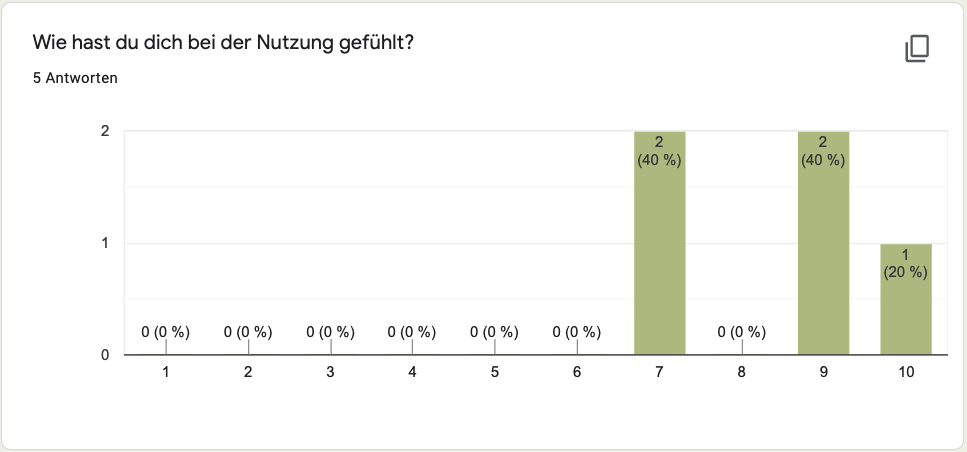
\includegraphics[width=1\textwidth]{images/Stimmungsbild.png}
    \caption[Evaluierung - Stimmungsbild]{Evaluierung - Stimmungsbild}
    \label{fig:EvaluierungStimmungsbild}
\end{figure}
Anhand des Stimmungsbilds aus der letzten Evaluierung lässt sich jedoch abschließend feststellen, dass die erarbeitete Gestaltungslösung, trotz fehldener Features und kleinere Anpassungsmöglichkeiten, sowie Fehler und Verbesserungsmöglichkeiten in der Erfahrung des Prototypen durch die Limitierung von Figma, die Nutzer zufrieden stellt.
\newpage
\chapter{Fazit}
\label{cha:Fazit}
Anhand der Durchführung des Prozesses zur Gestaltung gebrauchstauglicher interaktiver Systeme - entnommen aus der DIN-EN-ISO 9421-210 \citep{DINISO_2010} - setzte sich diese Arbeit im Wesentlichen mit der Zufriedenstellung der Nutzer mit einem System für den Austausch von traditionellen und kulturellen Rezepten auseinander. Dabei wurden die Schritte aus dem Vorgehensmodell der Norm durchlaufen und fortlaufend evaluiert. Final wurde eine Umfrage durchgeführt, um ein Stimmungsbild der Nutzer zu erfassen und auswerten zu können. \\

Aufgrund der geringen Anzahl an Teilnehmenden an der finalen Evaluierung können keine allgemeingültigen Schlussfolgerungen gezogen werden.
Die Abdeckung der repräsentativen Nutzergruppe für die Evaluierungsprozesse und deren Anzahl ist sehr wichtig, da sich statistische Ausreißer bei Umfragen mit kleineren Gruppen größer auf das Endergebnis auswirken als bei einer größeren Teilnehmerzahl. 
Zu erkennen war die Auswirkung auf das Endergebnis durch größere Teilnehmerzahl, besonders bei der Erarbeitung einer Gestaltungslösung für ein gedrucktes Rezept, um den Styleguide für das System zu erarbeiten (siehe \ref{subsec:styleguide}). Daher sollten kommende Arbeiten auf fortlaufende Evaluierung bestehen und auf mehr Resourcen zurückgreifen, um aussagekräftigere Schlüsse ziehen zu können. \\

Die Ergebnisse der Arbeit zeigen, dass die Anzahl der Iterationen wesentlichen Einfluss mit der Ergonomie und Zufriedenheit der Nutzer hat. Die weniger oft ausgeführten Evaluationszyklen - während der Konzeption der Wireframes - sorgte für Probleme bei der Erstellung der Gestaltungslösung in Form von Schleifen. Daher sollten die Evaluationen bereits, wie auch von der DIN Norm empfohlen, stets zu Beginn eingeplant und vor allem konsequent durchgeführt werden. \\

Aus den Ergebnissen lässt sich schließlich ableiten, dass die DIN Norm, für die Gestaltung von ergonomischen interaktiven Systemen sowie für den Austausch von kulturellen und traditionellen Rezepten geeignet ist, da die durchschnittliche Zufriedenheit der befragten Nutzer bei 8 von 10 Punkten lag. Die negativen Bewertungen von Teilsystemen ließen sich auf Mängel in der Durchführung des Prozesses oder Vorbereitung der Evaluierung zurückführen und belasten daher nicht die Bewertung der DIN Norm im Hinblick auf dieses System. \\

Somit wurde gezeigt, dass die DIN Norm für den Prozess zur Gestaltung gebrauchstauglicher interaktive Systeme geeignet ist. Sie sollte strikter befolgt werden, um Schleifen in den Arbeitsprozessen zu vermeiden beziehungsweise früher durchzuführen, um den Arbeitsaufwand zu reduzieren sowie die Zufriedenheit von Nutzern zu steigern.
Durch den Fokus auf die Gestaltung des Systems wurde im Rahmen dieser Projektarbeit nicht genauer auf die Auswahl der Frameworks für die Umsetzung eingegangen. Diese stellt jedoch einen bedeutenden Ansatz für zukünftige Arbeiten dar.
% wird fortlaufend auf der Basis benutzerzentrierter Evaluierung vorangetrieben
% Überblick über den Aufbau der Arbeit, Ergebnisse der einzelnen Kapitel
% Ergebnisse und Forschungsfrage in Beziehung setzen: „Harmonie zwischen den aus dem Thema abgeleiteten Fragestellung(en) und den im Schlussteil ausgewiesenen Ergebnissen, die Antworten zu diesen Fragestellungen geben“
% Ergebnisse in Forschungskontext einordnen, Geltungsbereich kritisch einschätzen (vgl. Winter 2004: 76); selbstkritische Reflexion, Kritikpunkte, Fehlstellen und Beschränkungen
% Schlussfolgerungen, offene Fragen (vgl. Samac, Prenner & Schwetz 2014: 74), Vorschläge für weitere Forschung: „future research“ (vgl. Franck 2004: 199)

\newpage
\pagenumbering{Roman}
\setcounter{page}{4}
%Erzeugt ein Abbildungsverzeichnis
	\listoffigures
	%Fügt die Zeile "`Abbildungsverzeichnis"' als Chapter ins Inhaltsverzeichnis ein
	\addcontentsline{toc}{chapter}{Abbildungsverzeichnis}
\newpage
	
	%Erzeugt ein Tabellenverzeichnis
	\listoftables
	%Fügt die Zeile "`Tabellenverzeichnis"' als Chapter ins Inhaltsverzeichnis ein
	\addcontentsline{toc}{chapter}{Tabellenverzeichnis}
\newpage

% To change the title from References to Bibliography:
\renewcommand\refname{Literaturverzeichnis}

%Paket für ein deutsches Literaturverzeichnis

\bibliographystyle{natdin} % or try natplain or unsrtnat
\bibliography{literatur} % refers to literatur.bib

	%Fügt die Zeile "`Literaturverzeichnis"' als Chapter ins Inhaltsverzeichnis ein
	\addcontentsline{toc}{chapter}{Literaturverzeichnis}
\newpage

%!TEX root = ../main.tex
\chapter*{Eidesstattliche Erklärung}
\addcontentsline{toc}{chapter}{Eidesstattliche Erklärung}

Ich versichere, die von mir vorgelegte Arbeit selbständig verfasst zu haben.\\ \\
Alle Stellen, die wörtlich oder sinngemäß aus veröffentlichten oder nicht veröffentlichten Arbeiten anderer entnommen sind, habe ich als entnommen kenntlich gemacht. Sämtliche Quellen und Hilfsmittel, die ich für die Arbeit benutzt habe, sind angegeben.\\ \\
Die Arbeit hat mit gleichem Inhalt bzw. in wesentlichen Teilen noch keiner anderen Prüfungsbehörde vorgelegen.
\vspace{1.5cm}
\\
Gummersbach, \today
\vspace{1cm}
\\
\begin{figure}[!ht]
%	\centering
		\includegraphics[width=0.26\textwidth]{images/Joel_Mai_Unterschrift.jpg}
\end{figure}
\\
Joël Maximilian Mai
% chapter eidesstattliche_erklärung (end)

\end{document}